% !TeX program = lualatex
\documentclass[draft]{scrartcl}

\RequirePackage[british]{babel}  % Sprache
\RequirePackage{csquotes}  % Anführungszeichen

\RequirePackage{geometry}  % Seitenlayout (insbesondere Ränder)

\RequirePackage{amsmath, amssymb, amsthm}  % mathematische Grundlagen
\let\mathbbold\mathbb  % speichere herkömmliche Buchstaben mit Doppelstrich und Serifen
\RequirePackage[intlimits]{mathtools}  % stellt u. a. \DeclarePairedDelimiter zur Verfügung + weitere Verbesserungen für amsmath
\RequirePackage[math-style=ISO, bold-style=ISO, partial=upright]{unicode-math}  % für kursive gr. Großbuchstaben und aufrechtes ∂ benützt
\let\mathbb\mathbbold  % kehre zu herkömmlichen Buchstaben mit Doppelstrich und Serifen zurück; neue Zeichen wie 1 mittels \symbb{1} verfügbar
\RequirePackage{xfrac}  % schräge Brüche; vor fontspec zu laden!

\RequirePackage[protrusion=true]{microtype}  % für hängende Interpunktion
\RequirePackage{tabularx}  % bessere Trenner und Zeilentypen
\makeatletter
\@ifclassloaded{beamer}{}{\RequirePackage[inline]{enumitem}}  % bessere Aufzählung (mit *-Variante für Aufzählungen innerhalb eines Textes); für 'beamer' ausgeschaltet
\makeatother

\PassOptionsToPackage{dvipsnames}{xcolor}
\RequirePackage{tikz} % Grafikpaket
\RequirePackage{tikzpagenodes}  % benötig für current page
\RequirePackage{pgfplots}  % tikz-Erweiterung
\pgfplotsset{compat=1.18}

\RequirePackage[ruled, lined, longend, nofillcomment, linesnumbered]{algorithm2e}

\RequirePackage{hyperref}  % klickbare Verweise
\RequirePackage[nameinlink, noabbrev]{cleveref}  % Namen in Verweisen

\RequirePackage{fixdif}  % bessere Ableitungsoperatoren; benötigt 'unicode-math'; nach 'hyperref' zu laden

\RequirePackage[backend=biber, style=numeric-comp, sortcites]{biblatex}  % Quellenverzeichnis
\addbibresource{../sources.bib}

\RequirePackage[toc, math, pangram]{blindtext}  % lorem ipsum dolor sit amet
\RequirePackage{todonotes}
% Maths & Algorithms.
\NewDocumentCommand{\af}{}{
	\frac{\euler}{\raisebox{0.3ex}{\(\scriptstyle\euler - 1\)}}
}
\NewDocumentCommand{\afconst}{}{
	\frac{\euler}{\raisebox{0.3ex}{\(\scriptstyle\euler - 1 + \USWsmallconstant\)}}
}
\NewDocumentCommand{\afinv}{}{
	\frac{\euler - 1 + \USWsmallconstant}{\raisebox{0.4ex}{\(\scriptstyle\euler\)}}
}
\NewDocumentCommand{\agents}{}{
	\symscr{A}
}
\NewDocumentCommand{\allallocs}{m m}{
	\symbf{X}_{#1}(#2)
}
\NewDocumentCommand{\alloc}{s O{} O{i}}{
	\symbf{x}\IfEmptyF{#3}{_{#3}}\IfEmptyTF{#2}{\IfBooleanT{#1}{^*}}{^{\IfBooleanT{#1}{*}#2}}
}
\NewDocumentCommand{\alloclen}{s O{} O{i}}{
	\smash[b]{\tau\IfEmptyF{#3}{_{#3}}\IfEmptyTF{#2}{\IfBooleanT{#1}{^*}}{^{\IfBooleanT{#1}{*}#2}}}
}
\NewDocumentCommand{\asgd}{s m O{i}}{
	\IfBooleanTF{#1}{o}{\textsl{a}}\IfEmptyF{#3}{_{#3}}^{#2}
}
\NewDocumentCommand{\asgdbf}{s m O{i}}{
	\IfBooleanTF{#1}{o}{\makebox[\widthof{\textsl{a}}]{\textsbf{\textsl{a}}}}\IfEmptyF{#3}{_{#3}}^{#2}
}
\makeatletter
\let\asgdnbf\asgd
\@ifclassloaded{beamer}{\RenewDocumentCommand{\alertmath}{D<>{1-} m}{
	\alt<#1>{
		\usebeamercolor[fg]{alerted text}
		\let\asgd\asgdbf
		\boldsymbol{#2}
		\let\asgd\asgdnbf
		\usebeamercolor[fg]{normal text}
	}{
		#2
	}
}}{}
\makeatother
\NewDocumentCommand{\attopt}{m O{i}}{
	\mybar{0.95}{0.07em}{\symbf{x}}^*_{\smash{#2, #1}}
}
\NewDocumentCommand{\attoptlen}{m O{i}}{
	\smash{\mybar{1.2}{0.02em}{\tau}^{*}_{#2, #1}}
}
\NewDocumentCommand{\bipartitegraph}{}{
	G
}
\NewDocumentCommand{\colouringconstant}{}{
	c
}
\NewDocumentCommand{\genericitem}{O{}}{
	j\IfEmptyF{#1}{^{#1}}
}
\NewDocumentCommand{\genericset}{s O{}}{
	\symscr{S}\IfBooleanT{#1}{^*}\IfEmptyF{#2}{_{#2}}
}
\NewDocumentCommand{\goods}{}{
	\symscr{G}
}
\NewDocumentCommand{\goodsordered}{m O{i}}{
	\goods\IfEmptyF{#2}{_{#2}}^{\smash[t]{#1}}
}
\NewDocumentCommand{\goodsrem}{}{
	\symscr{G}^{\mathup{rem}}
}
\NewDocumentCommand{\lostset}{m O{i}}{
	\symscr{L}_{\smash{\IfEmptyF{#2}{#2, } #1}}
}
\NewDocumentCommand{\lostsetlen}{m O{i}}{
	\ell_{\smash{\IfEmptyF{#2}{#2, } #1}}
}
\NewDocumentCommand{\matching}{O{}}{
	\symscr{M}\IfEmptyF{#1}{_{\hspace{-.1em}#1}}
}
\NewDocumentCommand{\overlygooditem}{O{i}}{
	j^{+}\IfEmptyF{#1}{_{#1}}
}
\NewDocumentCommand{\overlygoodset}{O{i}}{
	\goods^{+}\IfEmptyF{#1}{_{#1}}
}
\NewDocumentCommand{\phasei}{}{%
	Ⅰ%
}
\NewDocumentCommand{\phaseii}{}{%
	Ⅱ%
}
\NewDocumentCommand{\phaseiii}{}{%
	Ⅲ%
}
\NewDocumentCommand{\remvalue}{O{i}}{
	u\IfEmptyF{#1}{_{#1}}
}
\NewDocumentCommand{\USWconstant}{}{
	C
}
\NewDocumentCommand{\USWsmallconstant}{}{
	\varepsilon
}
\NewDocumentCommand{\unluckyagents}{m}{
	\agents^-_{#1}
}
\NewDocumentCommand{\unluckyagentsalgo}{m}{
	\alpha
}
\NewDocumentCommand{\unluckyagentslen}{m}{
	a^-_{#1}
}
\NewDocumentCommand{\valuations}{O{} o O{i}}{
	v\IfEmptyF{#3}{_{#3}}\IfEmptyF{#1}{\paren[#2]{#1}}
}
\NewDocumentCommand{\weight}{O{i}}{
	\eta\IfEmptyF{#1}{_{#1}}
}
\NewDocumentCommand{\weights}{}{
	E
}

\SetKwFunction{maxweightmatching}{max\_weight\_matching}
\SetKwFunction{arballoc}{arbitrary\_allocation}

\NewDocumentCommand{\phaseisep}{}{\nonl\CommentSty{Phase \phasei:}\;}
\NewDocumentCommand{\phaseiisep}{}{\vspace{0.25em}\nonl\CommentSty{Phase \phaseii:}\;}
\NewDocumentCommand{\phaseiiisep}{}{\vspace{0.25em}\nonl\CommentSty{Phase \phaseiii:}\;}

% Texts.
\NewDocumentCommand{\CASC}{}{\abb{CASC}}
\NewDocumentCommand{\Gap}{}{\abb{Gap-Max-\liningnums{3}-Colouring}}
\NewDocumentCommand{\EFone}{}{\abb{EF\liningnums{1}}}
\NewDocumentCommand{\EFX}{}{\abb{EFX}}
\NewDocumentCommand{\ESW}{}{%
	\relax\ifmmode{\operatorname{ESW}}\else{\abb{MEP}}\fi%
}
\NewDocumentCommand{\No}{}{\abb{No}~instance}
\NewDocumentCommand{\NSW}{}{%
	\relax\ifmmode{\operatorname{NSW}}\else{\abb{MNP}}\fi%
}
\NewDocumentCommand{\OXS}{}{\abb{OXS}}
\NewDocumentCommand{\PO}{}{\abb{PO}}
\makeatletter
\NewDocumentCommand{\RepReMatch}{}{\@ifpackageloaded{libertinus}{\Lss02{RepReMɑtc\Lsalt{h}}}{RepReMatch}}
\NewDocumentCommand{\SMatch}{}{\@ifpackageloaded{libertinus}{SMɑtc\Lsalt{h}}{SMatch}}
\makeatother
\NewDocumentCommand{\SPLC}{}{\abb{SPLC}}
\NewDocumentCommand{\USW}{}{%
	\relax\ifmmode{\operatorname{USW}}\else{\abb{MUP}}\fi%
}
\NewDocumentCommand{\XOS}{}{\abb{XOS}}
\NewDocumentCommand{\Yes}{}{\abb{Yes}~instance}

\crefname{property}{property}{properties}
\Crefname{property}{Property}{Properties}
%%% General notation in math.
\mathtoolsset{mathic=true}  % italic correction (use \(..\) instead of $..$)

% A ⇔  (or other symbol) on the left side of an align environment without affecting the width of the formula.
% modelled after: https://tex.stackexchange.com/a/574795
\NewDocumentCommand{\liff}{O{\!\!\iff}}{
	\begin{tikzpicture}[baseline=(tmp.base), remember picture]
		\node[inner sep=0pt] (tmp) {\vphantom{}};
		\begin{scope}[overlay]
			\path (current page text area.west|-tmp.base)
			node[anchor=base west, inner sep=0pt, outer sep=0pt]{\(#1\)}
			;
		\end{scope}
	\end{tikzpicture}
}

% The same as above but with an additional horizontal shift.
\NewDocumentCommand{\liffsh}{m O{\!\!\iff}}{
	\begin{tikzpicture}[baseline=(tmp.base), remember picture]
		\node[inner sep=0pt] (tmp) {\vphantom{}};
		\begin{scope}[overlay]
			\path (current page text area.west|-tmp.base)
			node[anchor=base west, inner sep=0pt, outer sep=0pt, xshift=#1]{\(#2\)}
			;
		\end{scope}
	\end{tikzpicture}
}


% A tag on the right. To be used with 'leqno' option for amsmath
% taken from: https://tex.stackexchange.com/a/574795
\NewDocumentCommand{\rtag}{m}{
	\begin{tikzpicture}[baseline=(tmp.base), remember picture]
		\node[inner sep=0pt](tmp){\vphantom{1}};
		\begin{scope}[overlay]
			\path (current page text area.east|-tmp.base)
			node[anchor=base east,inner sep=0pt,outer sep=0pt]{(#1)}
			;
		\end{scope}
	\end{tikzpicture}
}


%%% Delimiters.
\DeclarePairedDelimiter{\abs}{\vert}{\vert}
\DeclarePairedDelimiter{\braces}{\{}{\}}
\DeclarePairedDelimiter{\brackets}{[}{]}
\DeclarePairedDelimiter{\ceil}{\lceil}{\rceil}
\DeclarePairedDelimiter{\floor}{\lfloor}{\rfloor}
\NewDocumentCommand{\given}{O{}}{\mathrel{#1\vert}}
\DeclarePairedDelimiter{\norm}{\lVert}{\rVert}
\DeclarePairedDelimiter{\paren}{\lparen}{\rparen}


%%% Operators.
% Cups with dots inside for disjoint unions.
% taken from: https://tex.stackexchange.com/questions/110976/is-a-cupdot-symbol-available-in-amsmath?noredirect=1&lq=1
\makeatletter
\providecommand*{\cupdot}{%
	\mathbin{%
		\mathpalette\@cupdot{}%
	}%
}
\newcommand*{\@cupdot}[2]{%
	\ooalign{%
		$\m@th#1\cup$\cr
		\sbox0{$#1\cup$}%
		\dimen@=\ht0 %
		\sbox0{$\m@th#1\cdot$}%
		\advance\dimen@ by -\ht0 %
		\dimen@=.5\dimen@
		\hidewidth\raise\dimen@\box0\hidewidth
	}%
}

\providecommand*{\bigcupdot}{%
	\mathop{%
		\vphantom{\bigcup}%
		\mathpalette\@bigcupdot{}%
	}%
}
\newcommand*{\@bigcupdot}[2]{%
	\ooalign{%
		$\m@th#1\bigcup$\cr
		\sbox0{$#1\bigcup$}%
		\dimen@=\ht0 %
		\advance\dimen@ by -\dp0 %
		\sbox0{\scalebox{2}{$\m@th#1\cdot$}}%
		\advance\dimen@ by -\ht0 %
		\dimen@=.5\dimen@
		\hidewidth\raise\dimen@\box0\hidewidth
	}%
}
\makeatother

% Cup with higher lower limit (to be used for textmode).
\providecommand*{\highbigcup}{%
	\mathop{\bigcup{}}
}

% Differential operators
\letdif*{\dif}{d}  % \d is redefined by fixdif. This line is just for renaming.
\letdif*{\diff}{updelta}  % * = spacing correction; perhaps remove the asterisks if changing the math font
\letdif*{\difp}{partial}
\newdif*{\D}{\mathrm{D}}
\letdif*{\grad}{nabla}
\letdif*{\nabla}{nabla}
\DeclareDocumentCommand{\laplacian}{s}{
	\IfBooleanTF{#1}{\mathdif*{\Delta}}{\nabla^2}
}

% Minima and maxima.
\DeclareMathOperator*{\argmax}{arg\,max}
\DeclareMathOperator*{\argmin}{arg\,min}


%%% Constants and specifiers.
\def\APX{\ensuremath{\mathcal{APX}}}
\def\euler{\ensuremath{\mathup{e}}}
\def\NP{\ensuremath{\mathcal{NP}}}
\def\P{\ensuremath{\mathcal{P}}}

% Sets of numbers.
\def\nat{\mathbb{N}}
\def\natzero{\mathbb{N}_{0}}
\def\natnozero{\mathbb{N}_{>0}}
\def\real{\mathbb{R}}
\def\realpos{\mathbb{R}^+}
\def\realposzero{\mathbb{R}_0^+}


%%% Power set.
\NewDocumentCommand{\powerset}{so}{
	\IfNoValueTF{#2}{
		\mathcal{P}
	}{
		\IfBooleanTF{#1}{
			\mathcal{P}\left(#2\right)
		}{
			\mathcal{P}(#2)
		}
	}
}



%%% Bachmann-Landau notation.
\def\bigo{\ensuremath{\mathcal{O}}} % TODO: Schreibweisen angleichen
\def\bigomega{\ensuremath{\upOmega}}


%%% Stochastic notation.
\NewDocumentCommand\Prob{sm}{\IfBooleanTF{#1}{\mathbb{P}\!\left[#2\right]}{\mathbb{P}[#2]}}
\NewDocumentCommand\Erw{sm}{\IfBooleanTF{#1}{\mathbb{E}\!\left[#2\right]}{\mathbb{E}[#2]}}
\NewDocumentCommand\Var{sm}{\IfBooleanTF{#1}{\operatorname{Var}\!\left[#2\right]}{\operatorname{Var}[#2]}}
\NewDocumentCommand\Cov{sm}{\IfBooleanTF{#1}{\operatorname{Cov}\!\left[#2\right]}{\operatorname{Cov}[#2]}}

\def\Unif{\mathfrak{U}}
\def\Norm{\mathfrak{N}}


%%% Abbreviation in texts.
\def\eg{\mbox{e.\thinskip g.}\@}  % mbox to prevent breaks
\def\ie{\mbox{i.\thinskip e.}\@}


%%% Notation in texts.
\def\pp{\nobreak pp}  % percentage points

\NewDocumentCommand{\OPT}{}{\abb{OPT}}
\NewDocumentCommand{\ALG}{}{\abb{ALG}}

\NewDocumentCommand{\caseintextfont}{}{}  % actually defined in theme.sty
\NewDocumentEnvironment{caseintext}{m m}{\par\smallskip\noindent{\caseintextfont Case #1 \Dash #2:}}{\par\smallskip}

% Thin spaces around en dash (\dash) and em dash(\Dash). Use only for English texts!
% taken from: https://tex.stackexchange.com/questions/268111/automated-spacing
\makeatletter
\DeclareRobustCommand{\thinskip}{\hskip 0.16667em\relax}
\def\endash{--}
\def\emdash{\endash-}
\def\d@sh#1#2{\unskip#1\thinskip#2\thinskip\ignorespaces}
\def\dash{\d@sh\nobreak\endash}
\def\Dash{\d@sh\nobreak\emdash}
\def\ldash{\d@sh\empty{\hbox{\endash}\nobreak}}
\def\rdash{\d@sh\nobreak\endash}
\def\Ldash{\d@sh\empty{\hbox{\emdash}\nobreak}}
\def\Rdash{\d@sh\nobreak\emdash}
\makeatother

% \DeclareRobustCommand\textsb[1]{{\libertineSB#1}}  % semi bold


%%% Tables.
% Column types for tabularx (X = justified)
\newcolumntype{L}{>{\raggedright\arraybackslash}X}  % left-aligned
\newcolumntype{C}{>{\centering\arraybackslash}X}  % centered
\newcolumntype{R}{>{\raggedleft\arraybackslash}X}  % right-aligned


%%% Algorithms.
% Removes line number for one line. Best use with \nosemic
% taken from: https://tex.stackexchange.com/a/153906
\makeatletter
\newcommand{\nosemic}{\renewcommand{\@endalgocfline}{\relax}}  % Drop semi-colon ;
\newcommand{\dosemic}{\renewcommand{\@endalgocfline}{\algocf@endline}}  % Reinstate semi-colon ;
\newcommand{\pushline}{\Indp}  % indent
\newcommand{\popline}{\Indm\dosemic}  % undent
\let\oldnl\nl
\newcommand{\nonl}{\renewcommand{\nl}{\let\nl\oldnl}}
\makeatother


%%% Junk for playing around.
\def\ABC{ABCDEFGHIJKLMNOPQRSTUVWXYZ}
\def\abc{abcdefghijklmnopqrstuvwxyz}


%%% APA seminar.
% Maths & algo.
\NewDocumentCommand{\agents}{}{
	\mathcal{A}
}
\NewDocumentCommand{\allallocs}{m m}{
	\mathbfit{X}_{#1}(#2)
}
\NewDocumentCommand{\alloc}{s O{} O{i}}{
	\mathbfit{x}\IfEmptyF{#3}{_{#3}}\IfEmptyTF{#2}{\IfBooleanT{#1}{^*}}{^{\IfBooleanT{#1}{*}#2}}
}
\NewDocumentCommand{\alloclen}{s O{} O{i}}{
	\smash{\tau\IfEmptyF{#3}{_{#3}}\IfEmptyTF{#2}{\IfBooleanT{#1}{^*}}{^{\IfBooleanT{#1}{*}#2}}}
}
\NewDocumentCommand{\asgd}{s m O{i}}{
	\IfBooleanTF{#1}{g}{h}\IfEmptyF{#3}{_{#3}}^{#2}
}
\NewDocumentCommand{\attopt}{m O{i}}{
	\bar{\mathbfit{x}}^*_{\smash{#2, #1}}
}
\NewDocumentCommand{\attoptlen}{m O{i}}{
	\smash{\bar{\tau}^*_{#2, #1}}
}
\NewDocumentCommand{\bipartitegraph}{}{
	G
}
\NewDocumentCommand{\colouringconstant}{}{
	c
}
\NewDocumentCommand{\genericset}{s O{}}{
	\mathcal{S}\IfBooleanT{#1}{^*}\IfEmptyF{#2}{_{#2}}
}
\NewDocumentCommand{\goods}{}{
	\mathcal{G}
}
\NewDocumentCommand{\goodsordered}{m O{i}}{
	\goods\IfEmptyF{#2}{_{\!#2}}^{\thinspace\smash{#1}}
}
\NewDocumentCommand{\goodsreleased}{m}{
	\goods^{\mathup{rel}}_{#1}
}
\NewDocumentCommand{\goodsrem}{}{
	\mathcal{G}^{\mathup{rem}}
}
\NewDocumentCommand{\lostset}{m O{i}}{
	\mathcal{L}_{\smash{\IfEmptyF{#2}{#2, } #1}}
}
\NewDocumentCommand{\lostsetlen}{m O{i}}{
	\ell_{\smash{\IfEmptyF{#2}{#2, } #1}}
}
\NewDocumentCommand{\matching}{O{}}{
	\mathcal{M}\IfEmptyF{#1}{_{\hspace{-.1em}#1}}
}
\NewDocumentCommand{\overlygooditem}{O{i}}{
	j^{+}\IfEmptyF{#1}{_{#1}}
}
\NewDocumentCommand{\overlygoodset}{O{i}}{
	\goods^{+}\IfEmptyF{#1}{_{\!#1}}
}
\NewDocumentCommand{\phasei}{}{%
	\relax\ifmmode{\mathup{I}}\else{I}\fi%
}
\NewDocumentCommand{\phaseii}{}{%
	\relax\ifmmode{\mathup{II}}\else{II}\fi%
}
\NewDocumentCommand{\phaseiii}{}{%
	\relax\ifmmode{\mathup{III}}\else{III}\fi%
}
\NewDocumentCommand{\remvalue}{O{i}}{
	u\IfEmptyF{#1}{_{#1}}
}
\NewDocumentCommand{\USWconstant}{}{
	C
}
\NewDocumentCommand{\unluckyagents}{m}{
	\agents^-_{#1}
}
\NewDocumentCommand{\unluckyagentsalgo}{m}{
	\alpha
}
\NewDocumentCommand{\unluckyagentslen}{m}{
	a^-_{#1}
}
\NewDocumentCommand{\valuations}{O{} o O{i}}{
	v\IfEmptyF{#3}{_{#3}}\IfEmptyF{#1}{\paren[#2]{#1}}
}
\NewDocumentCommand{\weight}{O{i}}{
	\eta\IfEmptyF{#1}{_{#1}}
}
\NewDocumentCommand{\weights}{}{
	\mathcal{W}
}

\SetKwFunction{maxweightmatching}{max\_weight\_matching}
\SetKwFunction{arballoc}{arbitrary\_allocation}

\NewDocumentCommand{\phaseisep}{}{\nonl\CommentSty{Phase \phasei:}\;}
\NewDocumentCommand{\phaseiisep}{}{\vspace{0.25em}\nonl\CommentSty{Phase \phaseii:}\;}
\NewDocumentCommand{\phaseiiisep}{}{\vspace{0.25em}\nonl\CommentSty{Phase \phaseiii:}\;}

% Texts.
\NewDocumentCommand{\abb}{m}{#1}  % actually defined in theme.sty

\NewDocumentCommand{\Gap}{}{\abb{Gap-Max-3-Colouring}}
\NewDocumentCommand{\ESW}{}{%
	\relax\ifmmode{\operatorname{ESW}}\else{\abb{ESW}}\fi%
}
\NewDocumentCommand{\No}{}{\abb{No}~instance}
\NewDocumentCommand{\NSW}{}{%
	\relax\ifmmode{\operatorname{NSW}}\else{\abb{NSW}}\fi%
}
\NewDocumentCommand{\RepReMatch}{}{\abb{RepReMatch}}
\NewDocumentCommand{\SMatch}{}{\abb{SMatch}}
\NewDocumentCommand{\USW}{}{%
	\relax\ifmmode{\operatorname{USW}}\else{\abb{USW}}\fi%
}
\NewDocumentCommand{\Yes}{}{\abb{Yes}~instance}

\crefname{property}{property}{properties}
\Crefname{property}{Property}{Properties}
%%% Font.
%\RequirePackage{libertine}
\RequirePackage[regular]{newcomputermodern}  % newest version of Computer Modern (regular: display weight)
\NewDocumentCommand{\abb}{m}{#1}  % abbreviations

% Logic notation.
\let\oldforall\forall
\renewcommand{\forall}{\oldforall \, }

\let\oldexist\exists
\renewcommand{\exists}{\oldexist \: }

\newcommand\existsnot{\oldexist! \: }

% Links.
\hypersetup{
	colorlinks,
	bookmarksopen,
	bookmarksnumbered,
	linkcolor=black,
	plainpages=false,
	hypertexnames=false,
	citecolor=blue!80!black,
	urlcolor=red,
	pdfdisplaydoctitle=true,
}

%% Set style of operators.
%% taken from: https://tex.stackexchange.com/questions/219417/how-to-change-the-default-font-of-math-operators/219427#219427
%\DeclareSymbolFont{sansops}{T1}{\sfdefault}{m}{n}
%\SetSymbolFont{sansops}{bold}{T1}{\sfdefault}{b}{n}
%
%\makeatletter
%\renewcommand\operator@font{\mathgroup\symsansops}
%\makeatother


%%% Page style.
\geometry{margin=3cm}

% Title page.
\setkomafont{publishers}{}  % \publishers in normal font


%%% Environments in roman style with bold title.
\theoremstyle{definition}
\newtheorem{definition}{Definition}
%\AfterEndEnvironment{definition}{\noindent\ignorespaces}
\newtheorem{example}{Example}
\newtheorem{condition}{Condition}
\newtheorem{problem}{Problem}


%%% Environments in italic style with bold title.
\theoremstyle{plain}
\newtheorem{theorem}{Theorem}
\newtheorem{proposition}{Proposition}
\newtheorem{lemma}{Lemma}
\newtheorem{corollary}{Corollary}
\newtheorem{observation}{Observation}
\newtheorem{conjecture}{Conjecture}


%%% Environments in roman style with italic title.
\theoremstyle{remark}
\newtheorem{remark}{Remark}
\newtheorem{annotation}{Annotation}
\newtheorem{claim}{Claim}
\newtheorem*{note}{Note}  % No numbering
\newtheorem{case}{Case}
\newtheorem{acknowledgment}{Acknowledgment}
\newtheorem{conclusion}{Conclusion}


%%% Algorithms.
\DontPrintSemicolon
\SetKwComment{tct}{{\footnotesize\(\rhd\)}\,}{}


%%% PDF options.
\hypersetup{
	pdfdisplaydoctitle=true,
}

\titlehead{Algorithms and Complexity Group\hfill Summer Semester \oldstylenums{2023} \\ Institute for Computer Science \\ Goethe University Frankfurt}
\subject{Seminar Approximation Algorithms}
\title{ANSWuSVþ(U)M}
%\subtitle{Seminar Approximation Algorithms}
\author{Zeno Adrian Weil}
\publishers{Supervisor: Dr Giovanna Varricchio}
\publishers{\begin{tabular}{r @{~}l}
	Examiner: & Prof Dr Martin Hoefer \\
	Supervisor: & Dr Giovanna Varricchio
\end{tabular}}
\date{\oldstylenums{\today}}

\makeatletter
\hypersetup{
	pdfauthor=\@author,
	pdftitle=\@title,
	pdfsubject=\@subject,
}
\makeatother

\begin{document}
	\maketitle

	\begin{abstract}
		\lipsum[6-8]
	\end{abstract}

	\listoftodos

	\section{Introduction}
\label{sec:intro}

\subsection{Motivation}
\label{subsec:intro:motivation}

The study of distributing goods amongst several recipients is an interdisciplinary field, pursued scientifically as early as the 1940s~\cite{the_problem_of_fair_division}.
It is interesting both computationally (how to distribute fast) and qualitatively (how to distribute well).
Its areas of application are manifold:
\begin{itemize}
	\item
	For industrial procurement, the preferences of buyers and sellers need be appropriately captured and real-world constraints on goods and services be taken into account~\cite{survey}.

	\item
	Mobile Edge Computing denotes a technique where mobile devices compete for computational and storage capabilities of physically close servers.
	However, the participation of users and the provision of the serves has to be incentivised and monetised~\cite{edge_computing_auction, edge_computing_report}.

	\item
	Many production sites, machines, etc. are required for manufacturing, and the tasks between them must be scheduled efficiently.
	Disturbances must be quickly paid heed to~\cite{survey}.

	\item
	Water is a crucial resource, and even hostile countries must come to mutual agreements on the withdrawal from contested rivers~\cite{water_management}.
\end{itemize}


\subsection{Preliminaries}
\label{subsec:intro:prelim}

In this seminar paper, we focus on unsharable and indivisible goods, which we term \emph{items}.
The recipients of those items are termed \emph{agents}.
The distributions of items amongst agents are modelled through allocations.
\begin{definition}
	Let~\(\goods\) be a set of \(m\) items and~\(\agents\) be a set of \(n\) agents.
	An \emph{allocation} is a tuple \(\alloc[][] = (\alloc)_{i \in \agents}\) of \emph{bundles} \(\alloc \subset \goods\) such that each item is element of exactly one bundle, \ie, \(\bigcup_{i \in \agents} \alloc = \goods\) and \(\alloc \cap \alloc[][i'] = \emptyset\) for all \(i \neq i'\).
	An item~\(j \in \goods\) is \emph{assigned} to agent \(i \in \agents\) if \(j \in \alloc\) holds.
\end{definition}

The satisfaction of an agent \(i\) with her bundle \(\alloc\) is measured by her \emph{valuation function}~\(\valuations\), which assigns each item set a real value.
We always assume that valuation functions are monotonically non-decreasing, \ie, \(\valuations[\genericset[1]] \le \valuations[\genericset[2]]\), \(\forall \genericset[1] \subset \genericset[2] \subset \goods\), and normalised, \ie, \(\valuations[\emptyset] = 0\).
Note that this implies non-negativity, \ie, \(\valuations[\genericset] \ge 0\), \(\forall \genericset \subset \goods\).
Besides fulfilling these properties, the valuation functions can come from a plethora of function families.
We discuss additive and submodular functions in greater detail.
\begin{description}
	\item[Additive]
	The valuation \(\valuations[\genericset]\) of an agent \(i\) for any item set \(\genericset \subset \goods\) is the sum of the valuations of the individual items \(j \in \genericset\) in set \(\genericset\), that is, \(\valuations[\genericset] = \sum_{j \in \genericset} \valuations[\{j\}]\).

	Additive functions are fairly simple but also useful, and many expansions exist~\cite{satiation_in_fisher_markets_and_approx_of_nsw, APNSWuSVþUM}.

	\item[Submodular]
	Let \(\valuations[\genericset[1] \given \genericset[2]] \coloneq \valuations[\genericset[1] \cup \genericset[2]] - \valuations[\genericset[2]]\) denote the marginal valuation of agent~\(i\) for an item set \(\genericset[1] \subset \goods\) over a disjoint set \(\genericset[2] \subset \goods\).
	This valuation function satisfies the submodularity constraint \(\valuations[\{j\} \given \genericset[1] \cup \genericset[2]] \le \valuations[\{j\} \given \genericset[1]]\), \(\forall \{j\}, \genericset[1], \genericset[2] \subset \goods\).

	Submodular valuation functions, which encompass the additive ones, have the property that the gain from assigning new items decreases with increasing bundle size.
	Diminishing returns are a common phenomenon in economics, making submodular functions worthwhile to study~\cite{inapprox_results_for_combi_auctions_with_submod_utility_funcs}.
	Their relations to matroids~\cite{submodular_low_value, approximating_nsw_under_rado_valuations, opt_approx_for_the_submod_nsw_in_the_value_oracle_model} make them interesting from a theoretical point of view, too.
\end{description}
In a slight abuse of notation, we sometimes omit curly braces delimiting a set, so we write \(\valuations[j_1, j_2, \dots]\) instead of \(\valuations[\{j_1, j_2, \dots\}]\) for example.

In order to measure and maximise the overall satisfaction of all agents, one needs to combine their valuations.
Several options arise here;
common choices are the utilitarian social welfare, that is the sum of all valuations~\cite{inapprox_results_for_combi_auctions_with_submod_utility_funcs, survey, APNSWuSVþUM, water_management, edge_computing_auction}, and the egalitarian social welfare, that is the minimum of all valuations~\cite{survey, APNSWuSVþUM}.
We consider a third one, the Nash social welfare.
\begin{problem}
	\label{prob:nsw}
	Given a set \(\goods\) of items and a set \(\agents\) of agents with valuation functions \(\valuations \colon \powerset[\goods] \to \realposzero\) and weights \(\eta_i \in \realpos\) for all agents \(i \in \agents\), the \emph{maximum Nash social welfare problem (\NSW)} is to find an allocation \(\alloc*[][]\) which maximises the weighted geometric mean of valuations, that is,
	\begin{equation*}
		\alloc*[][] \overset{!}{=} \smashoperator{\argmax_{\alloc[][] \in \allallocs{\scriptstyle\agents\kern1pt}{\goods}}} \braces{ \NSW(\alloc[][]) }
		\quad\text{with~}
		\NSW(\alloc[][]) \coloneq \paren[\Big]{ \smashoperator{\prod_{i \in \agents}} \valuations[\alloc]^{\,\textstyle\weight} }{}^{\textstyle 1 / \sum_{i \in \agents} \weight}
	\end{equation*}
	where \(\allallocs{\agents}{\goods}\) is the set of all possible allocations.
	The problem is called \emph{symmetric} if all agent weights \(\weight\) are equal, and \emph{asymmetric} otherwise.
\end{problem}

For the techniques employed in later sections, it is beneficial to consider the logarithmic Nash social welfare, that is,
\vspace{-1.5ex}
\begin{equation}
	\log \NSW(\alloc[][])
	= \frac{1}{\sum_{i \in \agents} \weight} \cdot \sum_{i \in \agents} \weight \log \valuations[\alloc] \mperiod[,]
\end{equation}
which is a sum instead of a product.
The Nash social welfare strikes a middle ground between the utilitarian and egalitarian social welfare, which focus on efficiency (height of overall satisfaction) and fairness (how agents value other agents' bundles), respectively.
In addition, it exhibits scale-freeness, that is invariance to the scales in which the valuations are expressed.
Even though the \NSW{} is \APX-hard, approximate solutions largely keep the properties of optimal allocations~\cite[see also \cref{rem:ef1}]{approximating_the_nsw_with_indiv_items, the_unreasonable_fairness_of_max_nsw, min_envy_and_max_avg_nsw_in_the_alloc_of_indiv_goods, finding_fair_and_efficient_allocs}.


\subsection[Related Work and Contribution]{Related Work and Contribution by \citeauthor{APNSWuSVþUM}}
\label{subsec:intro:contribution}

The research on the \NSW{} is rather young and less advanced than the research on other allocation problems.
As reference\footnotemark[1], for the submodular utilitarian social welfare problem, a hardness of \(\af\) was proven in \citeyear{inapprox_results_for_combi_auctions_with_submod_utility_funcs}~\cite{inapprox_results_for_combi_auctions_with_submod_utility_funcs}, and an \(\af\)-approximation algorithm was shown in \citeyear{opt_approx_for_the_submod_nsw_in_the_value_oracle_model}~\cite{opt_approx_for_the_submod_nsw_in_the_value_oracle_model} \Dash the additive case is trivially solvable through repeated maximum matchings anyway.
For the egalitarian social welfare problem, a randomised \((320 \sqrt{n} \log^3 n)\)-approximation algorithm for additive valuations~\cite{an_approx_algo_for_maxmin_fair_alloc_of_indiv_goods} and a \((2n-1)\)-approximation algorithm for submodular valuations~\cite{approx_algo_for_the_maxmin_alloc_problem} have been devised in \citeyear{an_approx_algo_for_maxmin_fair_alloc_of_indiv_goods} and \citeyear{approx_algo_for_the_maxmin_alloc_problem}, respectively.
These may not be the best algorithms though, as the best known lower bound on the approximation factor is \(2\)~\cite{allocating_indiv_goods}.

In contrast, for the symmetric additive \NSW{}, an approximation hardness of \(1.069\) was shown in \citeyear{satiation_in_fisher_markets_and_approx_of_nsw}~\cite{satiation_in_fisher_markets_and_approx_of_nsw}, but only n \(1.45\)-approximation algorithm has been found in \citeyear{finding_fair_and_efficient_allocs}~\cite{finding_fair_and_efficient_allocs}.
For the symmetric submodular \NSW, an \((m - n + 1)\)-approximation algorithm has been devised in \citeyear{min_envy_and_max_avg_nsw_in_the_alloc_of_indiv_goods}~\cite{min_envy_and_max_avg_nsw_in_the_alloc_of_indiv_goods}.
However, an approximation factor dependant on the number of items is not desirable as the number of items vastly exceeds the number of agents in many applications.
Moreover, both approaches exploit the symmetry of the studied problem and fail to extend to the asymmetric case.

\Citeauthor{APNSWuSVþUM}~\cite{APNSWuSVþUM} further the research by contributing two polynomial-time algorithms for the asymmetric \NSW.
The first one, \emph{\SMatch}, computes a \(2n\)-approximative allocation under additive valuation functions.
It does so by \textsl{s}martly \textsl{match}ing agents and items which make up the parts of a bipartite graph.
The second one, \emph{\RepReMatch}, computes a \(2n (\log_2 n + 3)\)-approximative allocation under submodular valuation functions.
It does so by \textsl{rep}eatedly computing \textsl{match}ings, which then get partly annulled, so that items can be \textsl{re}matched.


\subsection{Structure of the Report}
\label{subsec:intro:structure}

We present and analyse \SMatch{} in \cref{sec:smatch} and \RepReMatch{} in \cref{sec:reprematch}.
In \cref{sec:hardness}, we give an analysis on the hardness of the submodular \NSW.
\Cref{sec:conclusion} contains the summary, an overview of newly published work since 2020, and an outlook on open questions.


\footnotetext[1]{
	The overview is given on the state of research as it was roughly at the end of the year 2019, when \citeauthor{APNSWuSVþUM} published the version of their paper~\cite{APNSWuSVþUM} on which this seminar report is based.
}

	\section{SMatch}
\label{sec:smatch}

\subsection{Presentation of the Algorithm}
\label{subsec:smatch:presentation}

In the case of an equal number of agents and items, \ie, \(n = m\), the \emph{additive} \NSW{} can be solved exactly by finding a maximum matching on a bipartite graph with the sets of agents and of items as its parts;
the weight of an edge between agent \(i\) and item \(j\) would be the weighted logarithmic valuation of item \(j\) by agent \(i\), \ie{} \(\weight \log \valuations[j]\).
Should there be more items than agents, then it would seem natural to just repeat this process until all items are assigned.
The flaw of this idea is that such a greedy algorithm considers only the valuations of items in the current graph and perhaps the valuations of items already assigned.
As the following examples demonstrates, this leads to an algorithm with an approximation factor dependent on the number \(m\) of items.
\begin{example}
	\label{ex:bad_idea}
	There are \(m+1\) items \(\goods_{1}, \dots, \goods_{m+1}\) and two equally weighted agents \(\agents_{1}\) and \(\agents_{2}\).
	Agent \(\agents_{1}\) values item~\(\goods_{1}\) at \(m + \epsilon\) and all other items at~\(1\).
	Agent \(\agents_{2}\) values item~\(\goods_{1}\) at \(m\), item \(\goods_{m+1}\) at~\(1\) and all other items at~\(0\) (\cref{fig:bad_idea:instance}).
	In an optimal allocation \(\alloc*[][]\), item \(\goods_{1}\) would be assigned to agent~\(\agents_{2}\) and all other items to agent~\(\agents_{1}\), resulting in a Nash social welfare of \(\sqrt{m \cdot m} = m\) (\cref{fig:bad_idea:opt}).
	A repeated maximum matching algorithm would greedily assign item \(\goods_{1}\) to agent \(\agents_{1}\) and item \(\goods_{m+1}\) to agent \(\agents_{2}\) first.
	Even if all remaining items were going to be assigned to agent \(\agents_{1}\), the Nash social welfare would never surpass \(\smash{\sqrt{(2m + \epsilon - 1) \cdot 1}} < \sqrt{2m}\) (\cref{fig:bad_idea:alg}).
	The approximation factor of the output \(\alloc[][]\) therefore is at least \(\sqrt{m/2}\) and, thus, depends on the number of items.
\end{example}
The geometric mean is high when bundles are valued similarly, wherefore it may be beneficial to give an item to agents who cannot expect many more valuable ones in the future instead of to agents who value the item a bit more but do so for others as well.
This is known as the Pigou-Dalton transfer principle~\cite{sublin_approx_algo_for_nsw_with_xos_valuations}.

\begin{figure*}
	\tikzset{
		agent/.style = {draw, circle, font=\small, inner sep=1pt},
		item/.style = {draw, rectangle, font=\small},
		dots/.style = {font=\small},
		weight/.style = {font=\footnotesize},
		edgeopt/.style = {},
		edgealg/.style = {},
		edgegry/.style = {},
		node distance=12mm and 32mm,
		on grid
	}
	\def\allocationexample{
		\centering
		\begin{tikzpicture}
			% items
			\node[item] (i1)                       {\(\goods_{1}\)};
			\node[item] (i2)  [below=of i1]        {\(\goods_{2}\)};
			\node[item] (i3)  [below=of i2]        {\(\goods_{3}\)};
			\node[item] (im)  [below=of i3]        {\(\goods_{m}\)};
			\node[item] (im1) [below=of im]        {\(\goods_{m+1}\)};
			\node[dots] (id)  at ($(i3)!0.5!(im)$) {\(\vdots\)};
			% agents
			\node[agent] (a1) [left=of i1]  {\(\agents_1\)};
			\node[agent] (a2) [left=of im1] {\(\agents_2\)};
			% valuations
			\draw[edgealg] (a1) to node[weight, pos=.42,  above]      {\(m + \epsilon\)} (i1);
			\draw          (a1) to node[weight, pos=.42,  above]      {\(1\)}            (i2);
			\draw          (a1) to node[weight, pos=.39,  above]      {\(1\)}            (i3);
			\draw          (a1) to node[weight, pos=.32,  above]      {\(1\)}            (im);
			\draw[edgeopt] (a1) to node[weight, pos=.255, above]      {\(1\)}            (im1);

			\draw[edgeopt] (a2) to node[weight, pos=.26,  above left] {\(m\)}            (i1);
			\draw[edgegry] (a2) to node[weight, pos=.30,  above]      {\(0\)}            (i2);
			\draw[edgegry] (a2) to node[weight, pos=.37,  above]      {\(0\)}            (i3);
			\draw[edgegry] (a2) to node[weight, pos=.42,  above]      {\(0\)}            (im);
			\draw[edgealg] (a2) to node[weight, pos=.48,  above]      {\(1\)}            (im1);
		\end{tikzpicture}
	}
	\centering
	\begin{subfigure}{0.325\textwidth}
		\allocationexample
		\caption{%
			problem instance
		}
		\label{fig:bad_idea:instance}
	\end{subfigure}
	\hfill
	\begin{subfigure}{0.325\textwidth}
		\tikzset{
			edgealg/.style = {white},
			edgegry/.style = {white},
		}
		\allocationexample
		\caption{%
			\(\NSW(\alloc*[][]) = \sqrt{m \cdot m}\)
		}
		\label{fig:bad_idea:opt}
	\end{subfigure}
	\hfill
	\begin{subfigure}{0.325\textwidth}
		\tikzset{
			edgeopt/.style = {white},
			edgegry/.style = {white},
		}
		\allocationexample
		\caption{%
			\(\NSW(\alloc[][]) \le \sqrt{(2m + \epsilon - 1) \cdot 1}\)
		}
		\label{fig:bad_idea:alg}
	\end{subfigure}
	\caption{%
		Illustration of \cref{ex:bad_idea} with \(m+1\) items and two equally weighted agents, their valuations shown as edge labels.
		It demonstrates that naïvely repeated matching without consideration of the future leads to an allocation \(\alloc[][]\) which is at best a \(\smash{\sqrt{m/2}}\)-approximation of the optimum \(\alloc*[][]\), meaning the approximation factor depends on the number of items.
	}
	\label{fig:bad_idea}
\end{figure*}

The algorithm \SMatch{} (\cref{alg:smatch}) eliminates the flaw by first gaining foresight of the valuations of items assigned after the first matching, thereby achieving an approximation factor of \(2 n\) (\cref{th:smatch}).
For a fixed agent \(i\), order the items in descending order of valuations and denote the \(j\)th most liked item by~\(\goodsordered{j}\).
We assume a well-defined order, so items of equal valuation shall be ordered further by ID or something similar.
\SMatch{} does in fact repeatedly match items.
During the first matching, however, the edge weights are defined as \(\weight \log\paren[\big]{ \valuations[j] + \remvalue/n } \) for an edge between agent~\(i\) and item~\(j\).
The value \(\remvalue\) serves as estimation of the valuation of items assigned after the first matching (\cref{lem:lower_bound_later_items}) and is defined as
\vspace{-1.0ex}
\begin{equation}
	\label{eq:def_remvalue}
	\remvalue
	\coloneq \smashoperator{\min_{\substack{\genericset \subset \goods \\ \abs{\genericset} \le 2n}}} \,\{ \valuations[\goods \setminus \genericset] \}
	= \valuations[ \goodsordered{2n+1}, \dots, \goodsordered{m} ] \mperiod \vspace{-1.0ex}
\end{equation}
Note that the set \(\genericset\) realizing the minimum of \(\valuations[\goods \setminus \genericset]\) may have less than \(2n\) elements if there are less than \(2n\) items in total or if some items are valuated at \(0\).
From the second matching onwards, the edge weights are defined as \(\weight \log\paren[\big]{ \valuations[j] + \valuations[\alloc] }\), where~\(\alloc\) is the continuously updated bundle of agent \(i\).
The addend \(\valuations[\alloc]\) could lead to better allocations in applications but does not improve the approximation factor asymptotically and so is of no further interest in the analysis.

\begin{algorithm*}[t]
	\KwIn{%
		a set \(\goods\) of \(m\) items,
		a set \(\agents\) of \(n\) agents,
		additive valuation functions \(\valuations \colon \powerset[\goods] \to \realposzero\) and weights \(\weight \in \realpos\) for all agents \(i \in \agents\)
	}
	\KwOut{%
		a \(2n\)-approximation \(\alloc[][] = (\alloc)_{i \in \agents}\) of an optimal allocation
	}

	\(\remvalue \gets \valuations[ \goodsordered{2n+1}, \dots, \goodsordered{m} ] \quad\forall i \in \agents\)  \tct*{estimation of future valuations}
	\(\weights \gets \braces[\big]{\, \paren[\big]{ i, j, \weight \log\paren{ \valuations[j] + \remvalue/n } } \given[\bigm] i \in \agents, j \in \goods \,}\)  \tct*{weighted edges using estimation}
	\(\bipartitegraph \gets (\agents, \goods, \weights)\)  \tct*{bipartite graph}
	\(\matching \gets \maxweightmatching(\bipartitegraph)\)\;
	\(\alloc \gets \{\, j \given (i, j) \in \matching \,\} \quad\forall i \in \agents\)  \tct*{assign according to matching}
	\(\goodsrem \gets \goods \setminus \{\, j \given (i, j) \in \matching \,\}\)  \tct*{set of unassigned items}
	\While{\(\goodsrem \neq \emptyset\)}{
		\(\weights \gets \braces[\big]{\, \paren[\big]{ i, j, \weight \log\paren{ \valuations[j] + \valuations[\alloc] } } \given[\bigm] i \in \agents, j \in \goodsrem \,}\)  \tct*{weighted edges using only valuations}
		\(\bipartitegraph \gets (\agents, \goodsrem, \weights)\)\;
		\(\matching \gets \maxweightmatching(\bipartitegraph)\)\;
		\(\alloc \gets \alloc \cup \{\, j \given (i, j) \in \matching \,\} \quad\forall i \in \agents\)\;
		\(\goodsrem \gets \goodsrem \setminus \{\, j \given (i, j) \in \matching \,\}\)\;
	}
	\Return{\(\alloc[][]\)}

	\caption{%
		\SMatch{} for the asymmetric additive \NSW
	}
	\label{alg:smatch}
\end{algorithm*}


\subsection{Analysis of the Algorithm}
\label{subsec:smatch:analysis}

To calculate the approximation factor of \SMatch, we first need to establish a lower bound on the valuation of single items.
For convenience, we order the items of any set \(\genericset = \{ \genericitem[1], \genericitem[2], \dots \}\) in descreasing order of valuation, so that it holds \(\valuations[\genericitem[k]] \ge \valuations[\genericitem[k']]\) for all \(k < k'\).
Note that if set \(\genericset\) happens to be a bundle, then item \(\genericitem[k]\) was assigned according to the \(k\)th matching.
\begin{lemma}
	\label{lem:lower_bound_single_item}
	For each agent \(i \in \agents\) and her final bundle \(\alloc = \{\asgd{1}, \dots, \asgd{\alloclen}\}\), it holds \(\valuations[\asgd{t}] \ge \valuations[\goodsordered{tn}]\) for all \(t = 1, \dots, \alloclen\).
\end{lemma}
\begin{proof}
	Before the \(t\)th matching, no more than \((t-1) n\) items out of the \(tn\) most highly valued items \(\goodsordered{1}, \dots, \goodsordered{tn}\) have been assigned in previous matchings since at most~\(n\) many out of those items are assigned each time.
	Because of the \(t\)th matching, at most \(n-1\) more items could be assigned to other agents, leaving at least one item of \(\goodsordered{1}, \dots, \goodsordered{tn}\) attainable for agent \(i\).
	Since \(\valuations[\goodsordered{k}] \ge \valuations[\goodsordered{tn}]\) for all \(k \le tn\) by definition of \(\goodsordered{k}\), the lemma follows.
\end{proof}

We can now use \(\remvalue/n = \valuations[ \goodsordered{2n+1}, \dots, \goodsordered{m} ]/n\) to establish a lower bound on  the valuations of items assigned after the first matching.
\begin{lemma}
	\label{lem:lower_bound_later_items}
	For each agent \(i \in \agents\) and her final bundle \(\alloc = \{\asgd{1}, \dots, \asgd{\alloclen}\}\), it holds \(\valuations[ \asgd{2}, \dots, \asgd{\alloclen} ] \ge \remvalue/n\).
\end{lemma}
\begin{proof}
	By \cref{lem:lower_bound_single_item} and definition of \(\goodsordered{tn}\), every item \(\asgd{t}\) is worth at least as much as each item \(\goodsordered{tn+k}\) with \(k \in \{1, \dots, n\}\) and, consequently, its valuation \(\valuations[\asgd{t}]\) is at least as high as the mean valuation \(\frac{1}{n} \valuations[ \goodsordered{tn+1}, \dots, \goodsordered{tn + n} ]\).
	Also, it holds \(\alloclen n + n \ge m \) since agent~\(i\) gets assigned \(\alloclen \ge \floor*{\frac{m}{n}} \ge \frac{m}{n} - 1\) many items.
	This yields
	\vspace{-2.5ex}
	\begin{equation}
		\valuations[\asgd{2}, \dots, \asgd{\alloclen}]
		= \sum_{t=2}^{\alloclen \mathstrut} \valuations[\asgd{t}]
		\ge \sum_{t=2}^{\alloclen \mathstrut} \frac{1}{n} \valuations[ \goodsordered{tn+1}, \dots, \goodsordered{tn + n} ]
		\ge \frac{1}{n} \valuations[ \goodsordered{2n+1}, \dots, \goodsordered{m} ]
		= \frac{\remvalue}{n} \label{eq:lower_bound_later_items} \mperiod \vspace{-2.5ex}
	\end{equation}
\end{proof}

\begin{remark}
	In \cref{lem:lower_bound_later_items}, we assumed non-zero valuations for all items, hence the bundle lengths of \(\alloclen \ge \floor*{\frac{m}{n}}\).
	Of course, one would not assign items to agents who value them at zero in an actual program.
	Inasmuch as additional zeroes do not change the sum in \cref{eq:lower_bound_later_items}, \cref{lem:lower_bound_later_items} still holds.
\end{remark}

This allows us to calculate an approximation factor for \SMatch{} by comparing its output with an optimal allocation \(\alloc*[][]\).
\begin{theorem}
	\label{th:smatch}
	\SMatch{} has an approximation factor of \(2 n\).
\end{theorem}
\begin{proof}
	\Cref{lem:lower_bound_later_items} can be plugged into the logarithmic Nash social welfare:
	\vspace{-1.5ex}
	\begin{align}
		\log \NSW(\alloc[][])
		&= \frac{1}{\sum_{i \in \agents} \weight} \cdot \sum_{i \in \agents} \weight \log \valuations[\asgd{1}, \dots, \asgd{\alloclen}] \\
		&= \frac{1}{\sum_{i \in \agents} \weight} \cdot \sum_{i \in \agents} \weight \log \paren[\big]{ \valuations[\asgd{1}] + \valuations[\asgd{2}, \dots, \asgd{\alloclen}] } \\
		&\ge \frac{1}{\sum_{i \in \agents} \weight} \cdot \sum_{i \in \agents} \weight \log \paren[\big]{ \valuations[\asgd{1}] + \remvalue / n } \label{eq:smatch_maximising}
	\end{align}
	Notice that the first matching of \SMatch{} maximises the sum in \cref{eq:smatch_maximising}.
	Thus, assigning all agents~\(i\) their respective most highly valued item \(\asgd*{1}\) from an optimal bundle~\(\alloc* = \{ \asgd*{1}, \dots, \asgd*{\alloclen*} \}\) yields the even lower bound
	\vspace{-0.5ex}
	\begin{equation}
		\label{eq:smatch_approx_factor_lower_bound}
		\log \NSW(\alloc[][])
		\ge \frac{1}{\sum_{i \in \agents} \weight} \cdot \sum_{i \in \agents} \weight \log \paren[\big]{ \valuations[\asgd*{1}] + \remvalue / n } \mperiod
	\end{equation}
	Recall the definition of \(\remvalue\) from \cref{eq:def_remvalue}.
	Consider a slightly modified variant:
	\vspace{-0.5ex}
	\begin{equation}
		\remvalue = \valuations[\goods \setminus \genericset[i]]
		\textnormal{ with }
		\genericset[i] \coloneq \smashoperator{\argmin_{\substack{\genericset \subset \goods \\ \abs{\genericset} \le 2n}}} \{ \valuations[\goods \setminus \genericset] \}
	\end{equation}
	Now consider the set \(\genericset*[i]\) of the (at most) \(2n\) most highly valued items in the optimal bundle \(\alloc*\), that is,
	\vspace{-1.5ex}
	\begin{equation}
		\genericset*[i]
		\coloneq \smashoperator{\argmin_{\substack{\genericset \subset \alloc* \\ \abs{\genericset} \le 2n}}} \{ \valuations[\alloc* \setminus \genericset] \} \mperiod
	\end{equation}
	It holds \(\valuations[\asgd*{1}] \ge \frac{1}{2 n} \valuations[\genericset*[i]]\) because of \(\valuations[\asgd*{1}] \ge \valuations[j]\) for all items \(j \in \genericset*[i]\).
	Furthermore, it holds \(\remvalue = \valuations[\goods \setminus \genericset[i]] \ge \valuations[\alloc* \setminus \genericset[i]] \ge \valuations[\alloc* \setminus \genericset*[i]]\).
	We can insert these two inequalities into \cref{eq:smatch_approx_factor_lower_bound} and prove the theorem thereby:
	\vspace{-2.0ex}
	\begin{align}
		\log \NSW(\alloc[][])
		&\ge \frac{1}{\sum_{i \in \agents} \weight} \cdot \sum_{i \in \agents} \weight \log \paren[\bigg]{ \frac{\valuations[\genericset*[i]]}{2 n} + \frac{\valuations[\alloc* \setminus \genericset*[i]]}{n} } \\
		&\ge \frac{1}{\sum_{i \in \agents} \weight} \cdot \sum_{i \in \agents} \weight \log \paren[\bigg]{ \frac{\valuations[\alloc*]}{2n} } \\
		&= \log \paren[\bigg]{\frac{\NSW(\alloc*[][])}{2 n}}
	\end{align}
\end{proof}
The analysis is asymptotically tight~\cite[Section~6.3]{APNSWuSVþUM}.
It is possible to design an instance for the asym\-metric additive \NSW{} such that \SMatch{} achieves an approximation factor approaching \(n/2\).
It remains to be shown whether the symmetric additive \NSW{} leads to an asymptotically equally bad approximation factor.

\begin{remark}
	\label{rem:ef1}
	\SMatch{} produces \emph{fair} allocations which are \emph{envy-free up to one item (\EFone)}~\cite[Section~5.2]{APNSWuSVþUM}.
	An allocation~\(\alloc[][]\) is \EFone{} if, for every pair \((i, i') \in \agents^2\) of agents, one needs to remove at most one item from the bundle \(\alloc[][i']\) of agent \(i'\) such that agent \(i\) does not want to swap bundles.
	In other words, it holds \(\valuations[\alloc[][i]][][i] \ge \valuations[\alloc[][i']]\) or, if not, there is an item \(j \in \alloc[][i']\) such that \(\valuations[\alloc[][i]][][i] \ge \valuations[\alloc[][i'] \setminus \{j\}]\).

	However, \SMatch{} does not produce allocations which are \emph{Pareto-optimal (\PO)}, another popular fairness property~\cite[Remark~5.2]{APNSWuSVþUM}.
	An allocation~\(\alloc[][]\) is \PO{} if there is no other allocation \(\alloc[\prime][]\) where every agent is at least as well off and one agent is strictly better off, \ie, it does not hold \(\valuations[\alloc[\prime]] \ge \valuations[\alloc] \) for all agents \(i \in \agents\) and \(\valuations[\alloc[\prime][i']][][i'] > \valuations[\alloc[][i']][][i']\) for some agent \(i' \in \agents\).
\end{remark}

	\section{RepReMatch}
\label{sec:reprematch}

\begin{algorithm*}[!b]
	\KwIn{%
		a set \(\goods\) of \(m\) items,
		a set \(\agents\) of \(n\) agents,
		submodular valuation functions \(\valuations \colon \powerset[\goods] \to \realposzero\) and weights \(\weight \in \realpos\) for all agents \(i \in \agents\)
	}
	\KwOut{%
		\(2n(\log_2 n + 3)\)-approximation \(\alloc[\phaseiii][] = (\alloc[\phaseiii])_{i \in \agents}\) of an optimal allocation
	}
	\phaseisep
	\(\alloc[\phasei] \gets \emptyset \quad\forall i \in \agents\)  \tct*{initialise temporary allocation}
	\(\goodsrem \gets \goods\)  \tct*{set of unassigned items}
	\For{\(t \gets 1, \dots, \ceil{\log_2 n}+1\)}{
		\If{\(\goodsrem \neq \emptyset\)}{
			\(\weights \gets \braces[\big]{\, \paren[\big]{ i, j, \weight \log{ \valuations[j] } } \given[\bigm] i \in \agents, j \in \goodsrem \,}\)   \tct*{weighted edges using val. of single item}
			\(\bipartitegraph \gets (\agents, \goodsrem, \weights)\)  \tct*{bipartite graph}
			\(\matching \gets \maxweightmatching(\bipartitegraph)\)\;
			\(\alloc[\phasei] \gets \alloc[\phasei] \cup \{j\} \quad \forall(i, j) \in \matching\)  \tct*{assign temporarily according to matching}
			\(\goodsrem \gets \goodsrem \setminus \{\, j \given (i, j) \in \matching \,\}\)  \tct*{remove assigned items}
		}
	}
	\phaseiisep
	\(\alloc[\phaseii] \gets \emptyset \quad\forall i \in \agents\)   \tct*{put allocation \(\alloc[\phasei][]\) away \& initialise new, definite one}
	\While{\(\goodsrem \neq \emptyset\)}{
		\(\weights \gets \braces[\big]{\, \paren[\big]{ i, j, \weight \log{ \valuations[ \alloc[\phaseii] \cup \{j\} ] } } \given[\bigm] i \in \agents, j \in \goodsrem \,}\)   \tct*{valuation of item \& current bundle}
		\(\bipartitegraph \gets (\agents, \goodsrem, \weights)\)\;
		\(\matching \gets \maxweightmatching(\bipartitegraph)\)\;
		\(\alloc[\phaseii] \gets \alloc[\phaseii] \cup \{j\} \quad \forall(i, j) \in \matching\)  \tct*{assign definitely according to matching}
		\(\goodsrem \gets \goodsrem \setminus \{\, j \given (i, j) \in \matching \,\}\)\;
	}
	\phaseiiisep
	\(\goodsrem \gets \bigcup_{i \in \agents} \alloc[\phasei]\)  \tct*{release items assigned in phase~\phasei} \label{ln:goodsrem}
	\(\weights \gets \braces[\big]{\, \paren[\big]{ i, j, \weight \log{ \valuations[ \alloc[\phaseii] \cup \{j\} ] } } \given[\bigm] i \in \agents, j \in \goodsrem \,}\)   \tct*{valuation of item \& current bundle}
	\(\bipartitegraph \gets (\agents, \goodsrem, \weights)\)\;
	\(\matching \gets \maxweightmatching(\bipartitegraph)\)\;
	\(\alloc[\phaseiii] \gets \alloc[\phaseii] \cup \{j\} \quad\forall(i, j) \in \matching\)  \tct*{initialise final allocation \& assign def. according to matching}
	\(\goodsrem \gets \goodsrem \setminus \{\, j \given (i, j) \in \matching \,\}\)\;
	\(\alloc[\phaseiii][] \gets \arballoc( \agents, \goodsrem, \alloc[\phaseiii][], (\valuations)_{i \in \agents} )\)  \tct*{assign remainder of items arbitrarily}
	\Return{\(\alloc[\phaseiii][]\)}
	\caption{%
		\RepReMatch{} for the asymmetric submodular \NSW{}
	}
	\label{alg:reprematch}
\end{algorithm*}

\subsection{Presentation of the Algorithm}
\label{subsec:reprematch:presentation}

The algorithm \SMatch{} estimates the valuation of the lowest-value items by determining the set of highest-value items and then valuing the remaining items.
Unfortunately, this approach does not work for general \emph{submodular} valuation functions because taking the set of highest-value items away does not necessarily leave a set of lowest-value items.
In fact, it can be shown \cite{submodular_low_value} that determining the set of lowest-value items is approximable only within a factor of \(\bigomega(\sqrt{m / \ln m})\).

For this reason, the algorithm \RepReMatch{} (\cref{alg:reprematch}) relies on an approach with three phases, thereby achieving an approximation factor of \(2n(\log_2 n + 3)\) (\cref{th:reprematch}).
In phase~\phasei, a sufficiently big set of high-value items is determined through repeated matchings.
This phase serves merley to determine this set, so items are assigned temporarily only.
The edge weights reflect this by taking the valuations of just single items into account.

In phase~\phaseii, the remaining items are assigned definitely through repeated matchings.
Consequently, each edge weight is updated in each round to be the weighted logarithm of the valuation of both the respective item and the items assigned so far.

In phase~\phaseiii, the high-value items assigned in phase \phasei{} are released.
With the knowledge of phase~\phaseii, one maximum weight matching is calculated, and the matched items are assigned accordingly.
Similarly to the previous phase, each edge weight is the weighted logarithm of the valuation of both the respective item and the respective agent's bundle from phase \phaseii.
The remaining released items are assigned arbitrarily.

\subsection{Analysis of the Algorithm}
\label{subsec:reprematch:analysis}

We use the term \emph{round} to refer to the iterations of the loops in the phases~\phasei{} and~\phaseii.
For ease of notation, we refer to the moment right before the first iteration in phase~\phaseii{} as round \(0\).
We start by analysing phase~\phaseii{} as it is the first phase with definitive assignments.
To this end, we introduce two types of item sets.
\begin{definition}
	Let \(\alloc*\) be an optimal bundle of an agent \(i \in \agents\).
	For any round \(r \ge 1\) in phase~\phaseii, the set \(\lostset{r} \subset \alloc*\) of \emph{lost items} is the set of all items \(j \in \alloc*\) assigned to other agents \(i' \neq i\) in that round.
\end{definition}
\begin{definition}
	Let \(\alloc*\) be an optimal bundle of an agent \(i \in \agents\) and \(\alloc[\phaseii] = \{ \asgd{1}, \dots, \asgd{\alloclen[\phaseii]} \}\) be her bundle at the end of phase \phaseii.
	The set of \emph{optimal and attainable items} is defined as \(\attopt{0} \coloneq \alloc* \setminus \bigcup_{i' \in \agents} \alloc[\phasei][i']\) for round~\(0\) and as \(\attopt{r} \coloneq \attopt{r-1} \setminus ( \lostset{r} \cup \{\asgd{r-1}\} )\) for round \(r = 1, \dots, \alloclen[\phaseii]\).
\end{definition}
\noindent
We denote their sizes by \(\lostsetlen{r}\ \coloneq \abs{\lostset{r}}\) and \(\attoptlen{r} \coloneq \abs{\attopt{r}}\), respectively.
First, we give a lower bound on the valuations of optimal and attainable items.
\begin{lemma}
	\label{lem:induction}
	For each agent \(i \in \agents\) and her bundle \(\alloc[\phaseii] = \{ \asgd{1}, \dots, \asgd{\alloclen[\phaseii]} \}\), it holds in all rounds \(r = 2, \dots, \alloclen[\phaseii]\) of phase \phaseii{} that
	\begin{equation*}
		\valuations[ \attopt{r} \given \asgd{1}, \dots, \asgd{r-1} ] \ge \valuations[\attopt{1}] - \smashoperator{\sum_{r'=1}^{r-1}} \lostsetlen{r'+1} \cdot \valuations[ \asgd{r'} \given \asgd{1}, \dots, \asgd{r'-1} ] - \valuations[\asgd{1}, \dots, \asgd{r-1}] \mperiod
	\end{equation*}
\end{lemma}
\begin{proof}
	The proof by \citeauthor{APNSWuSVþUM}~\cite[13\psq]{APNSWuSVþUM} consists of a lengthy induction rich in formulae and case differentiations.
	This is why we give a different but intuitive approach.

	Writing the left-hand side of the lemma out in full gives
	\begin{equation}
		\valuations[ \attopt{r} \given \asgd{1}, \dots, \asgd{r-1} ]
		= \valuations[ \attopt{r} \cup \braces{ \asgd{1}, \dots, \asgd{r-1} } ] - \valuations[ \asgd{1}, \dots, \asgd{r-1} ] \mperiod[,]
		\label{eq:attopt_marginal}
	\end{equation}
	which explains the second subtrahend on the right-hand side.

	Next, we show a lower bound on \(\valuations[\attopt{r} \cup \braces{ \asgd{1}, \dots, \asgd{r-1} }]\).
%	The set \(\attopt{r}\) of optimal and attainable items in round~\(r\) is equal to the set \(\attopt{r}\) of optimal and attainable items in round \(r-1\) minus the set \(\lostset{r}\) of lost items of round~\(r\) and, possibly, the item \(\asgd{r-1}\) assigned in round \(r-1\) if it was optimal back then, \ie, \(\asgd{r-1} \in \attopt{r-1}\).
	The items which are optimal and attainable in round \(r\) were so in round~\(r-1\), too.
	Additionally, the optimal but lost items of round \(r\) were attainable in round \(r-1\) as well.
	The item \(\asgd{r}\) assigned to agent \(i\) in round \(r\) was also attainable in round \(r-1\) and may also be optimal.
	Therefore, it holds \(\paren{ \attopt{r} \cup \braces{\asgd{r-1}} } \supset \paren{ \attopt{r-1} \setminus \lostset{r} }\) and
	\begin{equation}
		\valuations[\attopt{r} \cup \braces{ \asgd{1}, \dots, \asgd{r-1} }]
		\ge \valuations[\attopt{r-1} \setminus \lostset{r} \cup \braces{ \asgd{1}, \dots, \asgd{r-2} }]
		\ge \valuations[\attopt{r-1} \cup \braces{ \asgd{1}, \dots, \asgd{r-2} }] - \valuations[\lostset{r}] \mperiod
		\label{eq:attopt_union}
	\end{equation}
	The second inequality makes intuitively sense when one thinks of diminishing returns:
	The gain from adding the set \(\lostset{r}\) to the items in \(\attopt{r-1} \cup \braces{ \asgd{1}, \dots, \asgd{r-1} }\) cannot be higher than its subtracted valuation over the empty set.
	If we now recursively apply \cref{eq:attopt_union}, we eventually arrive at
	\begin{equation}
		\valuations[\attopt{r} \cup \braces{ \asgd{1}, \dots, \asgd{r-1} }]
		\ge \valuations[\attopt{1}] - \sum_{r'=1}^{r-1} \valuations[\lostset{r'+1}] \mperiod
		\label{eq:attop_lost}
	\end{equation}

	Lastly, we give an upper bound on \(\valuations[\lostset{r'+1}]\).
	The valuation \(\valuations[j \given \asgd{1}, \dots, \asgd{r'-1}]\) of any item \(j \in \lostset{r'+1}\) in round \(r'\) cannot have been higher than \(\valuations[\asgd{r'} \given \asgd{1}, \dots, \asgd{r'-1}]\) as otherwise item \(\asgd{r'}\) would not have been assigned before item \(j\).
	From this follows
	\begin{equation}
		\valuations[\lostset{r'+1}] \le \lostsetlen{r'+1} \cdot \valuations[\asgd{r'} \given \asgd{1}, \dots, \asgd{r'-1}] \mperiod
		\label{eq:lost}
	\end{equation}
	Combining \cref{eq:attopt_marginal,eq:attop_lost,eq:lost} proves the lemma.
\end{proof}
%\begin{lemma}
%	\label{lem:induction}
%	For each agent \(i \in \agents\) and her bundle \(\alloc[\phaseii] = \{ \asgd{1}, \dots, \asgd{\alloclen[\phaseii]} \}\), it holds in all rounds \(r = 2, \dots, \alloclen[\phaseii]\) of phase \phaseii{} that
%	\begin{equation*}
%		\valuations[ \attopt{r} \given \asgd{1}, \dots, \asgd{r-1} ] \ge \valuations[\attopt{1}] - \lostsetlen{2} \cdot \valuations[\asgd{1}] - \smashoperator{\sum_{r'=2}^{r-1}} \lostsetlen{r'+1} \cdot \valuations[ \asgd{r'} \given \asgd{1}, \dots, \asgd{r'-1} ] - \valuations[\asgd{1}, \dots, \asgd{r-1}] \mperiod
%	\end{equation*}
%\end{lemma}
%\begin{proof}
%	We prove the lemma by induction on the number \(r\) of rounds.
%	In the beginning of the base case \(r=2\), agent \(i\) has already been assigned item \(\asgd{1}\).
%	For each of the optimal and attainable items~\(j \in \attopt{1}\) in round \(1\), the marginal valuation \(\valuations[j \given \emptyset]\) over the empty set was at most \(\valuations[\asgd{1} \given \emptyset]\), as otherwise item~\(\asgd{1}\) would not have been assigned first.
%	The marginal valuation \(\valuations[j \given \asgd{1}]\) over \(\{\asgd{1}\}\) is upper-bounded by \(\valuations[\asgd{1} \given \emptyset]\), too, due to the submodularity of valuations.
%	During round \(2\), a further \(\lostsetlen{2}\) of these items \(j\) are assigned to other agents, and item \(\asgd{2}\) is assigned to agent \(i\).
%	We can bound the marginal valuation of the remaining optimal and attainable items in round \(2\) in the following way:
%	\begin{caseintext}{1}{\(\asgd{1} \in \attopt{1}\)}
%		It holds \(\valuations[ \attopt{2} \given \asgd{1} ] = \valuations[ \attopt{2} \cup \{\asgd{1}\} ] - \valuations[\asgd{1}] = \valuations[\attopt{1} \setminus \lostset{2}] -  \valuations[\asgd{1}]\).
%	\end{caseintext}
%	\begin{caseintext}{2}{\(\asgd{1} \notin \attopt{1}\)}
%		Due to the monotonicity of the valuation functions, it holds \(\valuations[ \attopt{2} \cup \{\asgd{1}\} ] \ge \valuations[ \attopt{2} ]\) and, therefore, \(\valuations[ \attopt{2} \given \asgd{1} ] \ge \valuations[ \attopt{2} ] - \valuations[\asgd{1}] = \valuations[\attopt{1} \setminus \lostset{2}] -  \valuations[\asgd{1}]\).
%	\end{caseintext}
%	\noindent
%	In both cases, the base case is proven because
%	\begin{equation}
%		\valuations[ \attopt{2} \given \asgd{1} ]
%		\ge \valuations[\attopt{1} \setminus \lostset{2}] -  \valuations[\asgd{1}]
%		\ge \valuations[ \attopt{1} ] - \valuations[\lostset{2}] - \valuations[\asgd{1}]
%		\ge \valuations[ \attopt{1} ] - \lostsetlen{2} \cdot \valuations[\asgd{1}] - \valuations[\asgd{1}] \mperiod[,]
%	\end{equation}
%	where the second inequality is shown easily using an alternative definition of submodularity (\(\valuations[\genericset[1] \cup \genericset[2]] + \valuations[\genericset[1] \cap \genericset[2]] \le \valuations[\genericset[1]] + \valuations[\genericset[2]]\) with \(\genericset[1] = \attopt{1} \setminus \lostset{2}\) and \(\genericset[2] = \lostset{2} \)~\cite{inapprox_results_for_combi_auctions_with_submod_utility_funcs}), and the third inequality is due to all \(\lostsetlen{2}\) items \(j\) in set \(\lostset{2}\) not being assigned in round \(1\) although attainable, implying \(\valuations[j] \le \valuations[\asgd{1}]\).
%
%	For the induction hypothesis, we assume that the lemma holds true for all rounds up to some~\(r\).
%	In the induction step \(r \to r+1\), we differentiate the same two cases again:
%	\begin{caseintext}{1}{\(\asgd{r} \in \attopt{r}\)}
%		Again we exploit the submodularity of the valuation functions to obtain a lower bound on the marginal valuation of \(\attopt{r+1}\).
%		\begin{align}
%			\valuations[ \attopt{r+1} \given \asgd{1}, \dots, \asgd{r} ]
%			&= \valuations[ \attopt{r+1} \cup \{\asgd{r}\} \given \asgd{1}, \dots, \asgd{r-1} ] - \valuations[ \asgd{r} \given \asgd{1}, \dots, \asgd{r-1} ] \\
%			&= \valuations[ \attopt{r} \setminus \lostset{r+1} \given \asgd{1}, \dots, \asgd{r-1} ] - \valuations[ \asgd{r} \given \asgd{1}, \dots, \asgd{r-1} ] \\
%			&\ge \valuations[ \attopt{r} \given \asgd{1}, \dots, \asgd{r-1} ] - \valuations[ \asgd{r} \given \asgd{1}, \dots, \asgd{r-1} ] - \valuations[ \lostset{r+1} \given \asgd{1}, \dots, \asgd{r-1} ]
%		\end{align}
%	\end{caseintext}
%	\begin{caseintext}{2}{\(\asgd{r} \notin \attopt{r}\)}
%		At first, we use the monotonicity of the valuation functions to get the inequality
%		\begin{align}
%			\valuations[ \attopt{r} \given \asgd{1}, \dots, \asgd{r} ]
%			&= \valuations[ \attopt{r} \cup \{ \asgd{1}, \dots, \asgd{r} \} ] - \valuations[\asgd{1}, \dots, \asgd{r}] \\
%			&\ge \valuations[ \attopt{r} \cup \{ \asgd{1}, \dots, \asgd{r-1} \} ] - \valuations[\asgd{1}, \dots, \asgd{r}] \\
%			&= \begin{multlined}[t]
%				\paren[\big]{ \valuations[ \attopt{r} \cup \{ \asgd{1}, \dots, \asgd{r-1} \} ] - \valuations[\asgd{1}, \dots, \asgd{r-1}] } \\
%				- \paren[\big]{ \valuations[\asgd{1}, \dots, \asgd{r}] - \valuations[\asgd{1}, \dots, \asgd{r-1}] }
%			\end{multlined} \\
%			&= \valuations[ \attopt{r} \given \asgd{1}, \dots, \asgd{r-1} ] - \valuations[ \asgd{r} \given \asgd{1}, \dots, \asgd{r-1} ] \mperiod
%		\end{align}
%		Together with the submodularity of valuation, we obtain the same lower bound again:
%		\begin{align}
%			\valuations[ \attopt{r+1} \given \asgd{1}, \dots, \asgd{r} ]
%			&= \valuations[ \attopt{r} \setminus \lostset{r+1} \given \asgd{1}, \dots, \asgd{r} ] \\
%			&\ge \valuations[ \attopt{r} \given \asgd{1}, \dots, \asgd{r} ] - \valuations[ \lostset{r+1} \given \asgd{1}, \dots, \asgd{r} ] \\
%			&\ge \valuations[ \attopt{r} \given \asgd{1}, \dots, \asgd{r} ] - \valuations[ \lostset{r+1} \given \asgd{1}, \dots, \asgd{r-1} ] \\
%			&\ge \valuations[ \attopt{r} \given \asgd{1}, \dots, \asgd{r-1} ] - \valuations[ \asgd{r} \given \asgd{1}, \dots, \asgd{r-1} ] - \valuations[ \lostset{r+1} \given \asgd{1}, \dots, \asgd{r-1} ]
%		\end{align}
%	\end{caseintext}
%	In both cases, we can replace \(\valuations[ \attopt{r} \given \asgd{1}, \dots, \asgd{r-1} ]\) by the induction hypothesis and \(\valuations[ \lostset{r+1} \given \asgd{1}, \dots, \asgd{r-1} ]\) by \(\lostsetlen{r+1} \cdot \valuations[ \asgd{r} \given \asgd{1}, \dots, \asgd{r-1} ]\) to prove the induction step.
%	\begin{align}
%		\valuations[ \attopt{r+1} \given \asgd{1}, \dots, \asgd{r} ]
%		&\ge \begin{multlined}[t]
%			\valuations[\attopt{1}] - \lostsetlen{2} \cdot \valuations[\asgd{1}] - \smashoperator{\sum_{r'=2}^{r-1}} \lostsetlen{r'+1} \cdot \valuations[ \asgd{r'} \given \asgd{1}, \dots, \asgd{r'-1} ] \\
%			- \valuations[\asgd{1}, \dots, \asgd{r-1}] - \valuations[ \asgd{r} \given \asgd{1}, \dots, \asgd{r-1} ] - \lostsetlen{r+1} \cdot \valuations[ \asgd{r} \given \asgd{1}, \dots, \asgd{r-1} ]
%		\end{multlined} \\
%		&= \valuations[\attopt{1}] - \lostsetlen{2} \cdot \valuations[\asgd{1}] - \smashoperator{\sum_{r'=2}^{r}} \lostsetlen{r'+1} \cdot \valuations[ \asgd{r'} \given \asgd{1}, \dots, \asgd{r'-1} ] - \valuations[\asgd{1}, \dots, \asgd{r}]
%	\end{align}
%\end{proof}

The lemma can be used to find a lower bound on the marginal valuation of the items actually assigned in each round \(r\).
\begin{corollary}
	\label{cor:lower_bound_single_item}
	From \cref{lem:induction} follows
	\begin{equation*}
		\valuations[ \asgd{r} \given \asgd{1}, \dots, \asgd{r-1} ]
		\ge \paren[\Big]{ \valuations[\attopt{1}] - \smashoperator{\sum_{r'=1}^{r-1}} \lostsetlen{r'+1} \cdot \valuations[ \asgd{r'} \given \asgd{1}, \dots, \asgd{r'-1} ] - \valuations[\asgd{1}, \dots, \asgd{r-1}] } \Big/ \attoptlen{r} \mperiod
	\end{equation*}
%	\begin{equation*}
%		\valuations[ \asgd{r} \given \asgd{1}, \dots, \asgd{r-1} ]
%		\ge \paren[\Big]{ \valuations[\attopt{1}] - \lostsetlen{2} \cdot \valuations[\asgd{1}] - \smashoperator{\sum_{r'=2}^{r-1}} \lostsetlen{r'+1} \cdot \valuations[ \asgd{r'} \given \asgd{1}, \dots, \asgd{r'-1} ] - \valuations[\asgd{1}, \dots, \asgd{r-1}] } \Big/ \attoptlen{r} \mperiod
%	\end{equation*}
\end{corollary}
\begin{proof}
%	There are \(\attoptlen{0}\) optimal and attainable items in \(\attopt{0}\) at the start of phase~\phaseii.
%	Of those, \(\lostsetlen{l}\) many are assigned to other agents in each round \(l \le r\), and also some items \(\asgd{l}\) assigned to agent \(i\) may be optimal, whence an upper bound of \(\attoptlen{0} - \sum_{l=1}^{r} \lostsetlen{l}\) on the number \(\attoptlen{r}\) of items in the set \(\attopt{r}\).\todo{Possibly this whole estimation can be omitted as we ditch it in the following lemma.}

	Remember that valuation functions are monotonic if \(\valuations[\genericset[1]] \le \valuations[\genericset[2]]\) holds for all sets \(\genericset[1] \subset \genericset[2] \subset \goods\).
	Induction shows that there must be an item \(j \in \genericset[2]\) with valuation \(\valuations[j] \ge \valuations[\genericset[2]] / \abs{\genericset[2]}\), otherwise it would hold \(\valuations[\emptyset] > 0\).
	Applied to \cref{lem:induction}, this means that there must be an item \(j \in \attopt{r}\) with a marginal valuation of at least \(\valuations[ \attopt{r} \given \asgd{1}, \dots, \asgd{r-1} ] / \attoptlen{r}\)\mperiod{}
	As item \(\asgd{r}\) was the one to be assigned, its marginal valuation cannot be smaller.
\end{proof}

This, finally, enables us to give a lower bound on the valuation of the bundles \(\alloc[\phaseii]\).
\begin{lemma}
	\label{lem:lower_bound_all_items}
	For each agent \(i \in \agents\) and her bundle \(\alloc[\phaseii] = \{\asgd{1}, \dots, \asgd{\alloclen[\phaseii]}\}\), it holds
	\begin{equation*}
		\valuations[\asgd{1}, \dots, \asgd{\alloclen[\phaseii]}] \ge \valuations[\attopt{1}] / n \mperiod
	\end{equation*}
\end{lemma}
\begin{proof}
	In each round \(r = 1, \dots, \alloclen[\phaseii]\), \(\lostsetlen{r}\) optimal and attainable items of agent \(i\) are assigned to other agents.
	As there are \(n\) agents in total, \(n-1\) is an upper bound on \(\lostsetlen{r}\).
	Furthermore, after \(\alloclen[\phaseii]\) rounds, the number \(\attoptlen{\alloclen[\phaseii]}\) of optimal and attainable items is at most \(n-1 \le n\) elsewise agent \(i\) would have been assigned yet another item.
	Together with \cref{cor:lower_bound_single_item}, this proves the lemma:
	\begin{align}
		\valuations[\asgd{1}, \dots, \asgd{\alloclen[\phaseii]}]
		&= \valuations[\asgd{1}, \dots, \asgd{\alloclen[\phaseii] - 1}] + \valuations[ \asgd{\alloclen[\phaseii]} \given \asgd{1}, \dots, \asgd{\alloclen[\phaseii]} ] \\
		&\ge \begin{multlined}[t]
			\valuations[\asgd{1}, \dots, \asgd{\alloclen[\phaseii] - 1}] + \paren[\Big]{ \valuations[\attopt{1}] - \smashoperator{\sum_{r'=1}^{\alloclen[\phaseii]-1 \mathstrut}} \lostsetlen{r'+1} \cdot \valuations[ \asgd{r'} \given \asgd{1}, \dots, \asgd{r'-1} ] \\
				- \valuations[\asgd{1}, \dots, \asgd{\alloclen[\phaseii]-1}] } \Big/ \attoptlen{\alloclen[\phaseii]}  % \Big/ has better spacing than \Bigm/.
		\end{multlined} \\
		&\ge \begin{multlined}[t]
			\valuations[\asgd{1}, \dots, \asgd{\alloclen[\phaseii] - 1}] + \paren[\Big]{ \valuations[\attopt{1}] - \smashoperator{\sum_{r'=1}^{\alloclen[\phaseii]-1 \mathstrut}} (n-1) \valuations[ \asgd{r'} \given \asgd{1}, \dots, \asgd{r'-1} ] \\
				- \valuations[\asgd{1}, \dots, \asgd{\alloclen[\phaseii]-1}] } \Big/ n
		\end{multlined} \\
		&\ge \valuations[\asgd{1}, \dots, \asgd{\alloclen[\phaseii] - 1}] + \paren[\big]{ \valuations[\attopt{1}] - (n-1) \valuations[\asgd{1}, \dots, \asgd{\alloclen[\phaseii]-1}] - \valuations[\asgd{1}, \dots, \asgd{\alloclen[\phaseii]-1}] } \big/ n \\
		&= \valuations[\attopt{1}] / n
	\end{align}
%	\begin{align}
%		\valuations[\asgd{1}, \dots, \asgd{\alloclen[\phaseii]}]
%		&= \valuations[\asgd{1}, \dots, \asgd{\alloclen[\phaseii] - 1}] + \valuations[ \asgd{\alloclen[\phaseii]} \given \asgd{1}, \dots, \asgd{\alloclen[\phaseii]} ] \\
%		&\ge \begin{multlined}[t]
%			\valuations[\asgd{1}, \dots, \asgd{\alloclen[\phaseii] - 1}] + \paren[\Big]{ \valuations[\attopt{1}] - \lostsetlen{2} \cdot \valuations[\asgd{1}] - \smashoperator{\sum_{r'=2}^{\alloclen[\phaseii]-1 \mathstrut}} \lostsetlen{r'+1} \cdot \valuations[ \asgd{r'} \given \asgd{1}, \dots, \asgd{r'-1} ] \\
%				- \valuations[\asgd{1}, \dots, \asgd{\alloclen[\phaseii]-1}] } \Big/ \attoptlen{\alloclen[\phaseii]}  % \Big/ has better spacing than \Bigm/.
%		\end{multlined} \\
%		&\ge \begin{multlined}[t]
%			\valuations[\asgd{1}, \dots, \asgd{\alloclen[\phaseii] - 1}] + \paren[\Big]{ \valuations[\attopt{1}] - (n-1) \valuations[\asgd{1}] - \smashoperator{\sum_{r'=2}^{\alloclen[\phaseii]-1 \mathstrut}} (n-1) \valuations[ \asgd{r'} \given \asgd{1}, \dots, \asgd{r'-1} ] \\
%				- \valuations[\asgd{1}, \dots, \asgd{\alloclen[\phaseii]-1}] } \Big/ n
%		\end{multlined} \\
%		&\ge \valuations[\asgd{1}, \dots, \asgd{\alloclen[\phaseii] - 1}] + \paren[\big]{ \valuations[\attopt{1}] - (n-1) \valuations[\asgd{1}, \dots, \asgd{\alloclen[\phaseii]-1}] - \valuations[\asgd{1}, \dots, \asgd{\alloclen[\phaseii]-1}] } \big/ n \\
%		&= \valuations[\attopt{1}] / n
%	\end{align}
\end{proof}

After having obtained a lower bound on the valuation of items assigned in phase~\phaseii, we need a lower bound for phase~\phaseiii{} as well.
Therefor we introduce a third type of item set.
\begin{definition}
	Let \(\alloc* = \{ \asgd*{1}, \dots, \asgd{\alloclen*}\}\) be an optimal bundle of some agent \(i \in \agents\).
	The set of \emph{overly good} items is defined as \(\overlygoodset \coloneq \{\, j \in \goods \given \valuations[j] \ge \valuations[\asgd*{1}] \,\}\).
\end{definition}

\begin{lemma}
	\label{lem:overly_good_matching}
	In phase~\phaseiii, there exists a matching such that each agent \(i \in \agents\) is matched to one of her overly good items in the set \(\bigcup_{i' \in \agents} \alloc[\phasei][i']\) of released items.
\end{lemma}
\begin{proof}
	If all items were matched in phase~\phasei, \ie, \(\bigcup_{i' \in \agents} \alloc[\phasei][i'] = \goods\), then all optimal items are released in phase~\phaseiii{} and each agent can be matched to one;
	the lemma is proven immediately.
	If not, imagine for some~\(t\) that only the items assigned in the first~\(t\) rounds of phase~\phasei{} were released.
%	Denote the set of released items by \(\goodsreleased{t}\).
	Now choose some matching \(\matching[t]\) with the following properties:
	\begin{enumerate}
		\item
		\label[property]{enum:matching:agent}
		If for an agent \(i\) all overly good items were amongst the released items,
%		\ie, \(\overlygoodset \subset \goodsreleased{t}\),
		she gets matched with an overly good item \(j \in \overlygoodset\).

		\item
		\label[property]{enum:matching:max}
		The number of agents matched with one of their overly good items is maximal amongst all matchings fulfilling \cref{enum:matching:agent}.
	\end{enumerate}
	\Cref{enum:matching:agent} is always satisfiable as the union of \(k\) many sets \(\overlygoodset\) contains \(k\) different items~\(\asgd*{1}\), which can be matched with agents \(i\).
	\Cref{enum:matching:max} leads to all agents being matched with an overly good item when \(t = \ceil{\log_2 n}+1\), \ie{} the number of rounds in phase~\phasei, whence the lemma follows.
	To prove this, we denote by \(\unluckyagents{t}\) the set of agents who are \emph{not} matched with one of their overly good items, and show by induction on \(t\) that it holds \(\abs{\unluckyagents{t}} \le n/2^t\).

	In the base case \(t=1\), none of the items are assigned initially.
	Denote by \(\unluckyagentsalgo{1}\) the number of agents who were not assigned an overly good item in the first round of phase~\phasei.
	If \(\unluckyagentsalgo{1} \le n/2\), then a matching \(\matching[1]\) obviously exists and the base case is immediately proven.
	Otherwise, all items from at least \(\unluckyagentsalgo{1}\) many sets \(\overlygoodset\) got assigned to someone.
	Again:
	Each set \(\overlygoodset\) contains the item \(\asgd*{1}\), so the union of these sets contains at least~\(\unluckyagentsalgo{1}\) items which can be matched with at least \(\unluckyagentsalgo{1}\) agents upon release.
	This then leaves at most~\(n-\alpha < n/2\) agents not matched with an overly good item.

	For the induction hypothesis, we assume that the statement holds true for all rounds up to some \(t\).
	In the induction step \(t \to t+1\), by \cref{enum:matching:agent}, there is at least one unassigned, overly good item in each set \(\overlygoodset[i']\) of all agents \(i' \in \unluckyagents{t}\) at the start of round \(t+1\).
	Analogously to the base case, for at least half of those agents \(i'\), these unassigned items will be assigned to either them or someone else, and it can be argued accordingly.
	By the induction hypothesis, it holds \(\abs{\unluckyagents{t+1}} \le \abs{\unluckyagents{t}}/2 \le (n/2^t)/2 = n/2^{t+1}\).
\end{proof}

This allows us to calculate an approximation factor for \RepReMatch{} by comparing its output with an optimal allocation \(\alloc*[][]\).
\begin{theorem}
	\label{th:reprematch}
	\RepReMatch{} has an approximation factor of \(2n (\log_2 n + 3)\).
\end{theorem}
\begin{proof}
	By \cref{lem:overly_good_matching}, we can assign each agent \(i\) an overly good item \(\overlygooditem \in \overlygoodset\) in the beginning of phase~\phaseiii.
	\RepReMatch{} maximises the logarithmic Nash social welfare, so
	\begin{equation}
		\label{eq:reprematch_approx_factor_lower_bound}
		\log \NSW(\alloc[\phaseiii][])
		\ge \frac{1}{\sum_{i \in \agents} \weight} \cdot \sum_{i \in \agents} \weight \log \valuations[\overlygooditem, \asgd{1}, \dots, \asgd{\alloclen[\phaseii]}]
	\end{equation}
	is a lower bound on the logarithmic \NSW{} after the first matching in phase~\phaseiii, with \(\alloc[\phaseii] = \{ \asgd{1}, \dots, \allowbreak \asgd{\alloclen[\phaseii]} \}\) being the bundle of agent \(i\) at the end of phase~\phaseii.

	Item \(\overlygooditem\) was released in phase~\phaseiii, which means it was assigned in phase~\phasei, implying \(\overlygooditem \in \alloc* \setminus \attopt{0}\) and, subsequently, \(\overlygooditem \in (\alloc* \setminus \attopt{0}) \cup \lostset{1}\).
	Phase~\phasei{} runs for at most \(\ceil{\log_2 n}+1\) rounds, and at most~\(n\) items are assigned in each iteration.
	Therefore, at most \(n (\log_2 n + 2)\) optimal items are assigned in that phase, \ie, \(\abs{ \alloc* \setminus \attopt{0} } \le n (\log_2 n + 2)\).
	As in \cref{lem:lower_bound_all_items}, it also holds \(n \ge \lostsetlen{1} = \abs{\lostset{1}}\).
	Together with the monotonicity of the valuation functions, this yields
	\begin{equation}
		\label{eq:overly_good_item_lower_bound}
		\valuations[ \overlygooditem, \asgd{1}, \dots, \asgd{\alloclen[\phaseii]} ]
		\ge \valuations[\overlygooditem]
		\ge \frac{\valuations[ (\alloc* \setminus \attopt{0}) \cup \lostset{1} ][\big]}{n(\log_2 n + 3)}
	\end{equation}
	as lower bound on the valuations of bundles.
	Moreover, \cref{lem:lower_bound_later_items} and the monotonicity of the valuation functions functions yield
	\begin{equation}
		\label{eq:assigned_items_lower_bound}
		\valuations[ \overlygooditem, \asgd{1}, \dots, \asgd{\alloclen[\phaseii]} ]
		\ge \valuations[ \asgd{1}, \dots, \asgd{\alloclen[\phaseii]} ]
		\ge \frac{\valuations[\attopt{1}]}{n}
		\ge \frac{\valuations[\attopt{1}]}{n(\log_2 n + 3)}
		= \frac{\valuations[ \attopt{0} \setminus \lostset{1} ]}{n(\log_2 n + 3)}
	\end{equation}
	as yet another lower bound.
	The mean of \crefrange{eq:overly_good_item_lower_bound}{eq:assigned_items_lower_bound} and the monotonicity of the valuation functions give the concise lower bound
	\begin{align}
		\valuations[ \overlygooditem, \asgd{1}, \dots, \asgd{\alloclen[\phaseii]} ]
		&\ge \frac{1}{2} \paren*{ \frac{\valuations[ (\alloc* \setminus \attopt{0}) \cup \lostset{1} ][\big]}{n(\log_2 n + 3)} + \frac{\valuations[ \attopt{0} \setminus \lostset{1} ][\big]}{n(\log_2 n + 3)} } \\
		&\ge \frac{1}{2} \cdot \frac{ \valuations[ \paren{(\alloc* \setminus \attopt{0}) \cup \lostset{1}} \cup \paren{\attopt{0} \setminus \lostset{1}} ][\big] }{n(\log_2 n + 3)} \\
		&= \frac{ \valuations[\alloc*] }{2n(\log_2 n + 3)} \mperiod
	\end{align}
	We can insert this lower bound into \cref{eq:reprematch_approx_factor_lower_bound} and prove the theorem thereby:
	\begin{equation}
		\log \NSW(\alloc[\phaseiii][])
		\ge \frac{1}{\sum_{i \in \agents} \weight} \cdot \sum_{i \in \agents} \weight \log \paren[\bigg]{ \frac{ \valuations[\alloc*] }{2n(\log_2 n + 3)} }
		= \log \paren[\bigg]{ \frac{\NSW(\alloc*[][])}{2n(\log_2 n + 3)} }
	\end{equation}
\end{proof}

\todo[inline]{overly good → outstanding?}

	\section{Hardness of Approximation}
\label{sec:hardness}

\Citeauthor{APNSWuSVþUM}~\cite[Sction 4]{APNSWuSVþUM} provide the following hardness result.
\begin{theorem}
	The submodular \NSW{} is not approximable within a factor of \(\frac{\euler}{\euler - 1}\)\todo[info]{\(\mathbfit{i}\): Should it not be \(\frac{\euler - 1}{\euler} - \epsilon\)?} in polynomial time unless \(\P = \NP\).
\end{theorem}
\begin{proof}
	Consider the related \SW{} problem\footnotemark.
	\begin{problem}
		Given a set \(\goods\) of indivisible items and a set \(\agents\) of agents with monotonic, submodular valuation functions \(\valuations \colon \powerset[\goods] \to \real\) for all agents \(i \in \agents\), the \emph{symmetric submodular Social Welfare problem} (\SW) is to find an allocation maximising the sum of valuations, that is
		\begin{equation*}
			\argmax_{\alloc[][] \in \allallocs{n}{\goods}} \braces[\bigg]{ \smashoperator{\sum_{i \in \agents}} \valuations[\alloc] }
		\end{equation*}
		where \(\allallocs{n}{\goods}\) is the set of all possible allocations of the items in \(\goods\) amongst \(n\) agents.
	\end{problem}

	Note that this problem is identical to the symmetric submodular \NSW{} except for the sum in the target function instead of a product.
	We will exploit this fact to calculate the \NSW{} of instances for \SW.
	\citeauthor{inapproximability}~\cite{inapproximability} supply a polynomial-time reduction of \SW{} from the following problem:
	\begin{problem}
		Given a graph \(G = (V, E)\) and a constant \(\colouringconstant \le 1\), the \emph{\(\colouringconstant\)-\Gap{} problem} is to decide whether, for any 3-colouring of graph \(G\) which maximises the number of edges with different coloured endpoints, the number of such edges is~\(\abs{E}\) (\emph{\Yes}) or \(\colouringconstant \abs{E}\) and below (\emph{\No}).
	\end{problem}

%	Like the regular \abb{3-Colouring} problem, this problem is also \NP-hard.
	\begin{proposition}
		There exists a constant \(\colouringconstant \le 1\) such that the \(\colouringconstant\)-\Gap{} problem is \NP-hard.
	\end{proposition}
	Reducing an instance of the \(c\)-\Gap{} problem yields an instance of the symmetric submodular \SW{} problem with identical valuation functions.
	Its properties are as follows:
	\begin{description}
		\item[\Yes]
		The \SW{} is \(n \swconstant\) because every agent values her bundle at \(n\), whereby \(\swconstant\) is a constant depending on the input graph.
		The \NSW{} of the instance would be \(\swconstant\).

		\item[\No]
		The \SW{} is \(\frac{\euler - 1}{\euler} n \swconstant\).
		Applying the inequality of arithmetic and geometric means, \ie{}, \((x_1 + \dots + x_n)/n \ge \sqrt[n]{x_1 \cdot \dots \cdot x_n}\) for all nonnegative numbers \(x_1, \dots, x_n \in \realposzero\), reveals that the \NSW{} of the instance is at most \(\frac{\euler - 1}{\euler} \swconstant\).
	\end{description}
	Thereout follows that the submodular \NSW{} problem, even when symmetric and with identical valuation functions, cannot be approximated within a factor better than \(\frac{\euler}{\euler - 1}\);
	otherwise one could decide the \(c\)-\Gap{} problem in polynomial time by checking whether the corresponding \NSW{} instance has a value above \(\frac{\euler - 1}{\euler} \swconstant\).
\end{proof}

For a constant number of agents, \citeauthor{APNSWuSVþUM}~\cite[Section 5.1]{APNSWuSVþUM} describe a family \((A_{\epsilon})_{\epsilon > 0}\) of algorithms for the asymmetric submodular \NSW{} problem where each algorithm \(A_\epsilon\) achieves an approximation factor of \(\frac{\euler}{\euler - 1} + \epsilon\).

\footnotetext{
	\Citeauthor{APNSWuSVþUM} call it the \enquote{Allocation problem}.
	We changed the name to match the naming scheme of the \NSW{} problem and to avoid confusion, as both problems are about allocations.
}

	\section{Conclusion}

\begin{frame}{Summary \& Outlook}
	\adjustfortopitem
	\begin{itemize}
		\item
		allocation:
		partition of items amongst agents

		\item
		bundles valued using submodular valuation functions
		\begin{itemize}
			\item
			diminishing returns
		\end{itemize}

		\item
		Nash social welfare:
		weighted geometric mean of valuations

		\item
		approximation factor independent from \(m\)?

		\item
		simple, repeated matching fails because of missing foresight

		\item
		\RepReMatch:
		\(2n (\log n + 3)\)-approximative
		\begin{description}
			\item[Phase \phasei]
			finding enough outstanding items

			\item[Phase \phaseii]
			assigning remaining item

			\item[Phase \phaseiii]
			assigning outstanding items
		\end{description}
	\end{itemize}
	\beamerimage at (13cm, 5.50cm) {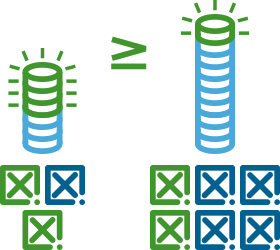
\includegraphics[height=1.45cm]{img/diminishingreturns}};
	\beamerimage at (13cm, 3.75cm) {
\includegraphics[height=1.45cm]{img/nvsm}};
	\beamerimage at (13cm, 2.00cm) {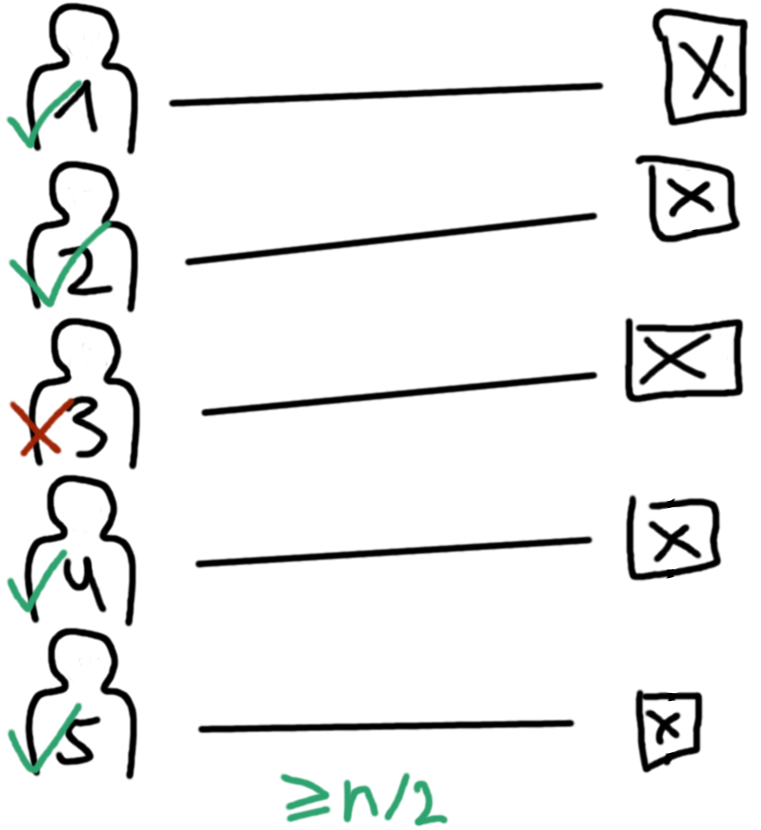
\includegraphics[height=1.45cm]{img/outstanding_1}};
	\beamerimage at (13cm, 0.25cm) {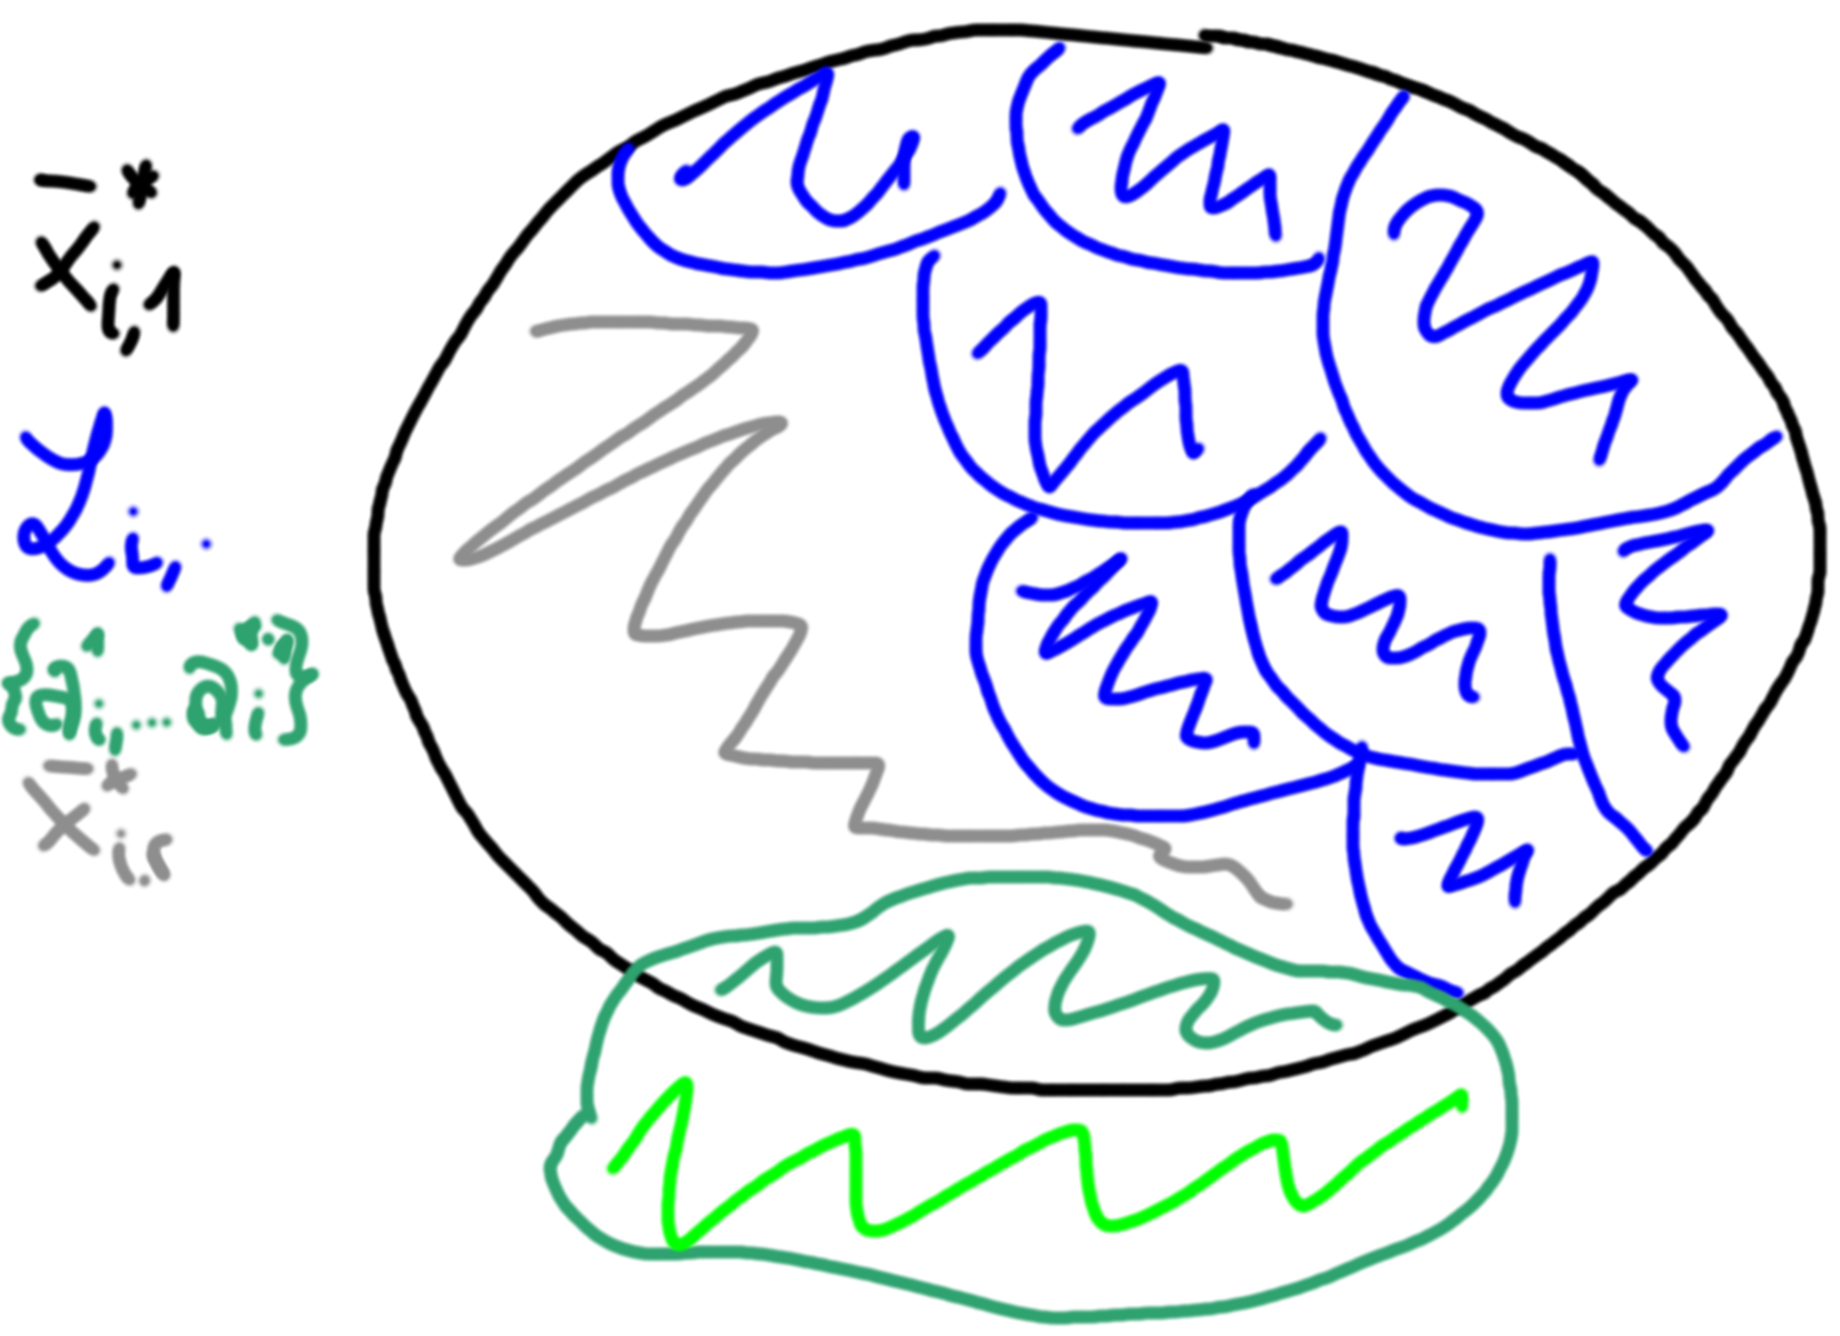
\includegraphics[height=1.45cm]{img/anal2_1}};
	\begin{minipage}{0.66\textwidth}
		\begin{block}{Any Room for Improvement?}
			Possibly! Lower bound of \(1.72\).
		\end{block}
	\end{minipage}
\end{frame}





\begin{frame}[c, plain, noframenumbering]
	\renewcommand{\insertsectionnumber}{!}
	\renewcommand{\insertsection}{End of Talk}
	\sectionpage
\end{frame}

	\clearpage

	\mybibliography
\end{document}